% Options for packages loaded elsewhere
\PassOptionsToPackage{unicode}{hyperref}
\PassOptionsToPackage{hyphens}{url}
\PassOptionsToPackage{dvipsnames,svgnames,x11names}{xcolor}
%
\documentclass[
  singlecolumn,
  9pt]{article}

\usepackage{amsmath,amssymb}
\usepackage{iftex}
\ifPDFTeX
  \usepackage[T1]{fontenc}
  \usepackage[utf8]{inputenc}
  \usepackage{textcomp} % provide euro and other symbols
\else % if luatex or xetex
  \usepackage{unicode-math}
  \defaultfontfeatures{Scale=MatchLowercase}
  \defaultfontfeatures[\rmfamily]{Ligatures=TeX,Scale=1}
\fi
\usepackage[]{libertinus}
\ifPDFTeX\else  
    % xetex/luatex font selection
\fi
% Use upquote if available, for straight quotes in verbatim environments
\IfFileExists{upquote.sty}{\usepackage{upquote}}{}
\IfFileExists{microtype.sty}{% use microtype if available
  \usepackage[]{microtype}
  \UseMicrotypeSet[protrusion]{basicmath} % disable protrusion for tt fonts
}{}
\makeatletter
\@ifundefined{KOMAClassName}{% if non-KOMA class
  \IfFileExists{parskip.sty}{%
    \usepackage{parskip}
  }{% else
    \setlength{\parindent}{0pt}
    \setlength{\parskip}{6pt plus 2pt minus 1pt}}
}{% if KOMA class
  \KOMAoptions{parskip=half}}
\makeatother
\usepackage{xcolor}
\usepackage[top=30mm,bottom=30mm,left=20mm,heightrounded]{geometry}
\setlength{\emergencystretch}{3em} % prevent overfull lines
\setcounter{secnumdepth}{-\maxdimen} % remove section numbering
% Make \paragraph and \subparagraph free-standing
\ifx\paragraph\undefined\else
  \let\oldparagraph\paragraph
  \renewcommand{\paragraph}[1]{\oldparagraph{#1}\mbox{}}
\fi
\ifx\subparagraph\undefined\else
  \let\oldsubparagraph\subparagraph
  \renewcommand{\subparagraph}[1]{\oldsubparagraph{#1}\mbox{}}
\fi


\providecommand{\tightlist}{%
  \setlength{\itemsep}{0pt}\setlength{\parskip}{0pt}}\usepackage{longtable,booktabs,array}
\usepackage{calc} % for calculating minipage widths
% Correct order of tables after \paragraph or \subparagraph
\usepackage{etoolbox}
\makeatletter
\patchcmd\longtable{\par}{\if@noskipsec\mbox{}\fi\par}{}{}
\makeatother
% Allow footnotes in longtable head/foot
\IfFileExists{footnotehyper.sty}{\usepackage{footnotehyper}}{\usepackage{footnote}}
\makesavenoteenv{longtable}
\usepackage{graphicx}
\makeatletter
\def\maxwidth{\ifdim\Gin@nat@width>\linewidth\linewidth\else\Gin@nat@width\fi}
\def\maxheight{\ifdim\Gin@nat@height>\textheight\textheight\else\Gin@nat@height\fi}
\makeatother
% Scale images if necessary, so that they will not overflow the page
% margins by default, and it is still possible to overwrite the defaults
% using explicit options in \includegraphics[width, height, ...]{}
\setkeys{Gin}{width=\maxwidth,height=\maxheight,keepaspectratio}
% Set default figure placement to htbp
\makeatletter
\def\fps@figure{htbp}
\makeatother
% definitions for citeproc citations
\NewDocumentCommand\citeproctext{}{}
\NewDocumentCommand\citeproc{mm}{%
  \begingroup\def\citeproctext{#2}\cite{#1}\endgroup}
\makeatletter
 % allow citations to break across lines
 \let\@cite@ofmt\@firstofone
 % avoid brackets around text for \cite:
 \def\@biblabel#1{}
 \def\@cite#1#2{{#1\if@tempswa , #2\fi}}
\makeatother
\newlength{\cslhangindent}
\setlength{\cslhangindent}{1.5em}
\newlength{\csllabelwidth}
\setlength{\csllabelwidth}{3em}
\newenvironment{CSLReferences}[2] % #1 hanging-indent, #2 entry-spacing
 {\begin{list}{}{%
  \setlength{\itemindent}{0pt}
  \setlength{\leftmargin}{0pt}
  \setlength{\parsep}{0pt}
  % turn on hanging indent if param 1 is 1
  \ifodd #1
   \setlength{\leftmargin}{\cslhangindent}
   \setlength{\itemindent}{-1\cslhangindent}
  \fi
  % set entry spacing
  \setlength{\itemsep}{#2\baselineskip}}}
 {\end{list}}
\usepackage{calc}
\newcommand{\CSLBlock}[1]{\hfill\break#1\hfill\break}
\newcommand{\CSLLeftMargin}[1]{\parbox[t]{\csllabelwidth}{\strut#1\strut}}
\newcommand{\CSLRightInline}[1]{\parbox[t]{\linewidth - \csllabelwidth}{\strut#1\strut}}
\newcommand{\CSLIndent}[1]{\hspace{\cslhangindent}#1}

\usepackage{cancel}
\usepackage[noblocks]{authblk}
\renewcommand*{\Authsep}{, }
\renewcommand*{\Authand}{, }
\renewcommand*{\Authands}{, }
\renewcommand\Affilfont{\small}
\usepackage{cancel}
\makeatletter
\@ifpackageloaded{caption}{}{\usepackage{caption}}
\AtBeginDocument{%
\ifdefined\contentsname
  \renewcommand*\contentsname{Table of contents}
\else
  \newcommand\contentsname{Table of contents}
\fi
\ifdefined\listfigurename
  \renewcommand*\listfigurename{List of Figures}
\else
  \newcommand\listfigurename{List of Figures}
\fi
\ifdefined\listtablename
  \renewcommand*\listtablename{List of Tables}
\else
  \newcommand\listtablename{List of Tables}
\fi
\ifdefined\figurename
  \renewcommand*\figurename{Figure}
\else
  \newcommand\figurename{Figure}
\fi
\ifdefined\tablename
  \renewcommand*\tablename{Table}
\else
  \newcommand\tablename{Table}
\fi
}
\@ifpackageloaded{float}{}{\usepackage{float}}
\floatstyle{ruled}
\@ifundefined{c@chapter}{\newfloat{codelisting}{h}{lop}}{\newfloat{codelisting}{h}{lop}[chapter]}
\floatname{codelisting}{Listing}
\newcommand*\listoflistings{\listof{codelisting}{List of Listings}}
\makeatother
\makeatletter
\makeatother
\makeatletter
\@ifpackageloaded{caption}{}{\usepackage{caption}}
\@ifpackageloaded{subcaption}{}{\usepackage{subcaption}}
\makeatother
\ifLuaTeX
  \usepackage{selnolig}  % disable illegal ligatures
\fi
\IfFileExists{bookmark.sty}{\usepackage{bookmark}}{\usepackage{hyperref}}
\IfFileExists{xurl.sty}{\usepackage{xurl}}{} % add URL line breaks if available
\urlstyle{same} % disable monospaced font for URLs
\hypersetup{
  pdftitle={Causal Diagrams for the Evolutionary Human Sciences: A Practical Guide},
  pdfauthor={Joseph A. Bulbulia},
  pdfkeywords={Directed Acyclic Graph, Causal
Inference, Confounding, Feedback, Interaction, Mediation, Moderation, Panel},
  colorlinks=true,
  linkcolor={blue},
  filecolor={Maroon},
  citecolor={Blue},
  urlcolor={Blue},
  pdfcreator={LaTeX via pandoc}}

\title{Causal Diagrams for the Evolutionary Human Sciences: A Practical
Guide}


  \author{Joseph A. Bulbulia}
            \affil{%
                  Victoria University of Wellington, New Zealand, School
                  of Psychology, Centre for Applied Cross-Cultural
                  Research
              }
      
\date{2023-11-19}
\begin{document}
\maketitle
\begin{abstract}
This article provides practical advice for creating causal diagrams. It
recommends aligning a graph's spatial layout with causation's temporal
order. I begin by reviewing assumptions foundational to causal
inference. I then explain how causal diagrams may be used to uncover
structurally sources of bias. I conclude by using chronologically
ordered diagrams to clarify widely misunderstood concepts causal
interaction, mediation, and dynamic longitudinal growth. Overall, this
guide hopes to equip evolutionary human scientists with tools and
understanding to enhance the rigour and clarity of their causal
inferences.
\end{abstract}
\subsection{Introduction}\label{introduction}

It is widely known that correlation does not imply causation.
Nevertheless, many human scientists report manifest correlations and use
hedging language that suggests causation. However, such reporting lacks
justification. Making matters worse, widely adopted strategies for
confounding control, such as regression adjustment, often enhance bias
(\citeproc{ref-mcelreath2020}{McElreath 2020}). Across many human
sciences, persistent confusion in the analysis and reporting of
correlations has greatly impeded scientific progress -- a causality
crisis (\citeproc{ref-bulbulia2022}{Bulbulia 2022}).

Incorporating causal diagrams, or ``directed acyclic graphs'', into
methodologically sound workflows can help to address the causality
crisis.\footnote{It is important to note that not every directed acyclic
  graph represents a causal structure. To qualify as such, a graph must
  meet specific criteria, including the Markov factorisation conditions,
  which are further elaborated in Part 2 of this discussion.}. Causal
diagrams are grounded in a system of formal mathematical proofs. However
they do not require extensive mathematical training. Causal diagrams are
broadly accessible and user-friendly.

Yet, causal inference differs from traditional data science by operating
within a theoretical framework focused on estimating counterfactual
contrasts---hypothetical outcomes under different scenarios. This
approach, termed `counterfactual data science', is grounded in specific
assumptions. Causal diagrams operate within this theoretical framework.
They clarify structural sources of bias and assist in understanding
conditions in which causal effects may be uniquely inferred from
observational data, based on the causal model and its assumptions. The
effectiveness of causal diagrams depends on the validity of these
assumptions; flawed or overly optimistic assumptions may lead to
misplaced confidence in causal inferences. The simplicity and
accessibility of causal diagrams make it tempting to use them to mask
unwarrented inferences. Causal diagrams are designed to clarify
structural sources of bias. However, if the underlying assumptions are
flawed or overly optimistic, causal diagrams may result in misplaced
confidence. Ideally, causal diagrams would discourage their users from
over-reaching.

There are many excellent introductions to causal diagrams
(\citeproc{ref-barrett2021}{Barrett 2021};
\citeproc{ref-cinelli2022}{Cinelli \emph{et al.} 2022};
\citeproc{ref-greenland1999}{Greenland \emph{et al.} 1999};
\citeproc{ref-hernuxe1n2023}{Hernán and Robins 2023};
\citeproc{ref-mcelreath2020}{McElreath 2020};
\citeproc{ref-pearl2009}{Pearl 2009a}; \citeproc{ref-rohrer2018}{Rohrer
2018}; \citeproc{ref-suzuki2020}{Suzuki \emph{et al.} 2020}).\footnote{An
  excellent resource is Miguel Hernan's free online course, here:
  \url{https://pll.harvard.edu/course/causal-diagrams-draw-your-assumptions-your-conclusions}.}
Here, I promote \emph{chronologically ordered causal diagrams}, in which
the spatial configuration and the labelling of nodes are aligned with
the temporal sequence of presumed causal events. By aligning the spatial
arrangement and labelling of nodes with the temporal sequence of
causatation, causal diagrams better mitigate the risk of overreaching.
They serve as a guide for researchers in both collecting appropriate
data and planning analyses that are congruent with the temporal dynamics
of the causal processes under study. A second benefit of this guide is
that it begins with an in-depth examination of the framework of
assumptions fundamental to counterfactual data science. This context is
crucial -- it is only with this setting that causal diagrams acquire
their utility. A third benefit is the application of causal diagrams to
clarifying widespread confusions in the analysis of multivariate
time-series data, where there is presently great confusion.

\textbf{Part 1} introduces the counterfactual framework for causal
inference as the appropriate theoretical setting for developing causal
diagrams. An understanding of these assumptions is a prerequisite for
effectively using causal diagrams. Before introducing causal diagrams,
it is vital to understand their role in this larger conceptual
framework. This framework, which I may be called ``counterfactual data
science,'' differs from standard data science.

\textbf{Part 2} examines the structures of \emph{confounding bias}. In
this part, the use of chronologically ordered causal diagrams is
introduced. Here, we find that chronological ordering not only clarifies
structural sources of bias and strategies that may adjust for it, but
also provides directives for data collection, revealing the importance
of collecting repeated measures on units over a time.

\textbf{Part 3} employs chronologically ordered causal diagrams to
clarify widely misunderstood concepts of causal interaction, mediation,
and longitudinal growth modelling. Here again, we find the benefit of
attending to chronology in the spatial layout of the graph.

\subsection{Part 1. Causal Inference as Counterfactual Data
Science}\label{part-1.-causal-inference-as-counterfactual-data-science}

Understanding how to frame causal questions is essential before
attempting to answer them (\citeproc{ref-hernuxe1n2016}{Hernán \emph{et
al.} 2016}). This section reviews the three core identification
assumptions necessary for causal inference.

\subsubsection{The Fundamental Problem of Causal
Inference}\label{the-fundamental-problem-of-causal-inference}

Consider an intervention, denoted as \(A\), and its effect, represented
as \(Y\). We assert that \(A\) causes \(Y\) if altering \(A\) leads to a
change in \(Y\) (\citeproc{ref-hume1902}{Hume 1902};
\citeproc{ref-lewis1973}{Lewis 1973}). The aim in causal inference is to
measure the difference in outcomes when the intervention (or treatment)
changes from one state to another.

However, a fundamental challenge arises. For any individual instance
where \(Y_i\) is observed, \(A_i\) will have only one level in the
required contrast. In a binary treatment scenario, we can observe either
\(Y_i|A_i = 1\) or \(Y_i|A_i = 0\), but never both simultaneously. This
means one of the outcomes necessary to determine the causal effect at
the individual level is counterfactual. The ``fundamental problem of
causal inference'' emerges because we can only see one treatment state
per individual at any given time (\citeproc{ref-holland1986}{Holland
1986}; \citeproc{ref-rubin1976}{Rubin 1976}). The outcome under the
unobserved or counterfactual treatment condition remains unknown. Thus,
causal inference grapples with a distinct missing data problem
(\citeproc{ref-edwards2015}{Edwards \emph{et al.} 2015};
\citeproc{ref-westreich2015}{Westreich \emph{et al.} 2015}). This issue
differs from typical missing data scenarios, where data could have been
recorded but were not. The missing information in causal analysis is
inherent to the nature of causal reasoning itself, which necessitates
contrasting the actual world with a hypothetical alternative. The
following discussion will explore the assumptions that allow us to
identify \emph{average} causal effects from the data.

\paragraph{Estimating Average Causal Effects in Evolutionary Human
Sciences}\label{estimating-average-causal-effects-in-evolutionary-human-sciences}

In the field of evolutionary human sciences, a central task is to
estimate average causal effects from observational data. This involves
discerning how a particular variable (such as a cultural belief) impacts
an outcome (such as social complexity). For instance, consider studying
the effect of belief in Big Gods (powerful, moralizing deities) on the
development of social complexity within societies.

In this context, the average treatment effect (ATE) aims to measure the
difference in social complexity between societies that believe in Big
Gods (treatment group) and those that do not (control group).
Mathematically, this can be expressed as:

\[
ATE = \mathbb{E}[Y(a)] - \mathbb{E}[Y(a^*)]
\]

Here, \(Y(a)\) represents the social complexity in societies believing
in Big Gods, and \(Y(a^*)\) represents social complexity in societies
without such beliefs.

The challenge in this analysis arises from the nature of observational
studies. In an ideal experiment, we could directly compare societies
before and after the introduction \emph{and} removal of Big God beliefs.
However, in reality, each society is observed only in one state --
either with or without the belief. This creates a missing data problem,
where we lack direct observations of the counterfactual scenario -- how
complex a society would be if its beliefs were different.

The formula addressing this missing data dilemma is:

\[
\delta = \underbrace{\big(\mathbb{E}[Y(1)|A = 1]\big)}_{\text{observed}} + \underbrace{\big(\mathbb{E}[Y(1)|A = 0]\big)}_{\text{unobserved}} - \underbrace{\big(\mathbb{E}[Y(0)|A = 0]\big)}_{\text{observed}}  - \underbrace{\big(\mathbb{E}[Y(0)|A = 1]\big)}_{\text{unobserved}}
\]

In plain terms, \(\delta\) (the average treatment effect) combines what
we can observe (social complexity in societies with or without Big Gods
belief) with what we cannot (the hypothetical social complexity in the
opposite scenarios).

Causal inference in evolutionary human science, therefore, must rely
statistical methods and assumptions to estimate these unobserved
effects. Conceptualising the ``full data'' -- which involves both the
observed data and the counterfactual data -- allows researchers to make
more informed conclusions about how cultural beliefs might shape
societal outcomes. Such a workflow takes researchers beyond the
limitations inherent in observational data. It is within such a
workflow, which might be called ``counterfactual data science'' that
causal diagrams find their application
(\citeproc{ref-bulbulia2023}{Bulbulia \emph{et al.} 2023}).

This approach, grounded in the ``potential outcomes'' framework,
provides a structured methodology for adressing fundamental
\emph{causal} questions in the evolutionary human science \footnote{There
  are different formulations of causality, and so arguably different
  frameworks. I use the singular ``the'' because, as used in applied
  research, the varieties of framework are mathematically equivalent.
  The variety I present here is called the ``potential outcomes''
  framework, which origins to works of Neyman
  (\citeproc{ref-neyman1923}{\textbf{neyman1923?}}), Rubin Rubin
  (\citeproc{ref-rubin1976}{1976}), and Robins Robins
  (\citeproc{ref-robins1986}{1986}).}, such as whether certain culturual
beliefs affect social evolution.

\subsubsection{Identification Assumption 1: Causal Consistency and
Treatment Effect
Heterogeneity}\label{identification-assumption-1-causal-consistency-and-treatment-effect-heterogeneity}

Causal consistency is essential in addressing the elusive missing data
problems inherent in causal inference.

Consider \(Y_i^{observed}|A_i\) as an individual's observed outcome
following treatment \(A_i\). Under the causal consistency assumption, we
can derive one of the counterfactual outcomes necessary for our causal
contrasts as follows:

\[
Y_i^{observed}|A_i = 
\begin{cases} 
Y_i(a^*) & \text{if } A_i = a^* \\
Y_i(a) & \text{if } A_i = a
\end{cases}
\]

This implies that the observed outcome at a given exposure level should
match the counterfactual outcome at that level. While it seems
straightforward to equate an observed outcome with its counterfactual,
the assumption becomes challenging because in most observational
settings there is likely to be \emph{treatment effect heterogeneity.}
Unlike an experiment where treatments are controlled, in observational
setting treatments may vary widely
(\citeproc{ref-vanderweele2009}{VanderWeele 2009a}).

Consider the previous example. Beliefs in Big Gods are not likely to be
uniform in their effects. Such beliefs vary over time and across
cultures in their intensity, interpretations, and institutional and
ritual embodiments. Such variation may significantly influence social
complexity. How can we estimate causal effects with such variable
``treatments.''

The theory causal inference under multiple versions of treatment reveals
that the problem of treatment effect heterogeneity is \emph{formally}
tractable.This theory demonstrates that even with multiple treatment
versions, consistent causal effects can be estimated if these versions
are conditionally independent of the outcomes
(\citeproc{ref-vanderweele2009}{VanderWeele 2009a},
\citeproc{ref-vanderweele2018}{2018};
\citeproc{ref-vanderweele2013}{VanderWeele and Hernan 2013}).
Specifically, if there are \(K\) different versions of treatment \(A\),
and there is no confounding for the effect of \(K\) on \(Y\) given
measured confounders \(L\), such that:

\[
K \coprod Y(k) | L
\]

or, equivalently:

\[
Y(k) \coprod K | L
\]

where \(\coprod\) denotes independence. If such independence is
achieved, causal consistency is attainable. In such settings, we may
think of \(A\) acts as a ``coarsened indicator'' for estimating the
causal effect of multiple treatment versions \(K\) on \(Y(k)\). Despite
this formal solution, doubts remain. How do we know whether the measured
covariates are sufficient to render the versions of treamtment
independent of the counterfactual outcomes? Even if we believe we have
such assurances, how shall we interpret a contrast that averages over
such variation? We set these problems aside for now. However, it is
important that researchers are aware that even when we successfully
employ causal diagrams to avert bias in estimating causal effects, we
might not be able to interpret the quantities that we are consistently
estimating. (For further discussions, see:
(\citeproc{ref-bulbulia2022}{Bulbulia 2022};
\citeproc{ref-hernuxe1n2008}{Hernán \emph{et al.} 2008};
\citeproc{ref-hernuxe1n2022a}{Hernán \emph{et al.} 2022};
\citeproc{ref-murray2021a}{Murray \emph{et al.} 2021}).)

For the moment, we note that the causal consistency assumption provides
a starting point for recovering the missing counterfactuals essential
for computing causal contrasts. It achieves this by identifying half of
these counterfactuals directly from observed data. The concept of
exchangeability, which we will explore next, offers a means to derive
the remaining half.

\subsubsection{Identification Assumption 2: (Conditional)
Exchangeability}\label{identification-assumption-2-conditional-exchangeability}

The concept of conditional exchangeability is central to causal
inference. In experimental settings, randomised assignment to
experimental conditions helps to ensure conditional exchangeability. In
observational settings we must work harder. The conditional
exchangeability assumption is met if, after accounting for observed
covariates, the assignment of treatment is random with respect to the
potential outcomes under that treatment. In simpler terms, it means that
once we control for certain known factors (covariates), the treatment
assignment should not systematically differ in groups with different
potential outcomes.

To put it into context, let us revisit the Big Gods and social
complexity example. If we assume both causal consistency (including no
interference) and positivity, achieving conditional exchangeability
would imply that if we hypothetically swapped societies between those
believing and not believing in Big Gods, the distribution of potential
social complexities under each belief system would not change. This
assumption is crucial for balancing the groups in terms of other factors
(confounders) that might influence both cultural beliefs in Big Gods and
social complexity.

By satisfying this assumption, along with the consistency and positivity
assumptions, we can treat the counterfactual observations as if they
were randomly assigned to the exposure conditions under which they were
observed. Essentially, meeting the conditional exchangeability
assumption is akin to replicating the conditions of a randomised
experiment within the confines of observational data.

Call \(L\) the set of measured covariates needed to ensure this
conditional independence. We use \(\coprod\) to denote independence. The
conditional exchangeability of potential outcomes given these covariates
\(L\) can be expressed as:

\[
Y(a) \coprod  A|L \quad \text{or equivalently} \quad A \coprod  Y(a)|L
\]

When this assumption holds, along with consistency and positivity, the
average treatment effect (ATE) on the difference scale can be computed:

\[
\delta_{ATE}  = \mathbb{E}[Y(a^*)|L = l] - \mathbb{E}[Y(a)|L = l]
\]

Ultimately, achieving conditional exchangeability allows researchers to
approximate the level of control found in randomised experiments, using
observational data. In fields such as cultural evolution, experimental
control is rarely feasible. For this reason we may only infer causal
effects in settings where the assumption of no unmeasured confounding is
credible.

\subsubsection{Identification Assumption 3:
Positivity}\label{identification-assumption-3-positivity}

The positivity assumption is satisfied if there is a non-zero
probability of receiving or not receiving the exposure within each level
of all covariates. In other words, within every stratum of every
covariate, the probability of each exposure value must be greater than
zero. Mathematically the positivity assumption is expressed:

\[
0 < \Pr(A=a|L=l)<1, ~ \forall a \in A, ~ \forall l \in L
\]

Causal inference encounters challenges without the satisfaction of the
positivity assumption, as the envisioning of causal contrasts hinges on
the potential for randomised assignment to interventions
(\citeproc{ref-westreich2010}{Westreich and Cole 2010}).

There are two types of positivity violations.

\begin{enumerate}
\def\labelenumi{\arabic{enumi}.}
\item
  \textbf{Random non-positivity}: where the exposure is conceivable, yet
  some potential observations, while theoretically possible, are absent
  within our data, we say that random non-positivity is violated. This
  situation often arises with continuous exposures, where certain
  realisations along the number line are naturally missing due to its
  infinite nature. Despite this, it remains possible to employ
  statistical models to estimate causal contrasts. Notably, random
  non-positivity is the only identifiability assumption that can be
  checked using data.
\item
  \textbf{Deterministic non-positivity:} where the exposure is
  inconceivable, we say that deterministic non-positivity is violated.
  For example, hysterectomy in biological males is said to violate
  deterministic non-positivity.
\end{enumerate}

\subsubsection{Summary Part 1}\label{summary-part-1}

To quantify causal effects requires converting observations from data
into \emph{counterfactual} causal contrasts. Causation itself is never
directly observed. Obtaining causal contrasts from observations in data
requires assumptions. The three fundamental assumptions of causal
inference are:

\begin{enumerate}
\def\labelenumi{\arabic{enumi}.}
\item
  \textbf{Causal Consistency}: exposures under comparison relate to
  well-defined interventions found in the data
  (\citeproc{ref-hernuxe1n2023}{Hernán and Robins 2023}) (see also:
  Chatton \emph{et al.} (\citeproc{ref-chatton2020}{2020})).
\item
  \textbf{Exchangeability}: after adjusted for measured covariates, the
  potential outcomes under all exposure levels are independent of the
  actual exposure level received (\citeproc{ref-hernuxe1n2023}{Hernán
  and Robins 2023}).
\item
  \textbf{Positivity:} the probability of receiving every exposure value
  within all strata of covariates exceeds zero
  (\citeproc{ref-hernuxe1n2023}{Hernán and Robins 2023}).
\end{enumerate}

In Part 1 we have reviewed the comprehensive framework of counterfactual
data science. We learned that \emph{if positivity is satisfied, the
counterfactual consistency assumption yields half of the required
counterfactual outcomes for inferring causal contrasts. Exchangeability
supplies the remaining half.} It is within this comprehensive framework
that causal diagrams find their utility. We use causal diagrams to
evaluate \emph{structural biases} arising from confounding, selection,
and measurement error (\citeproc{ref-hernuxe1n2023}{Hernán and Robins
2023}). Retaining a focus on these functions, within the framework of
counterfactual data science, helps to avert misapplications.

\subsection{Part 2.Applications of Chronologically Ordered Causal
Diagrams for Understanding Confounding
Bias}\label{part-2.applications-of-chronologically-ordered-causal-diagrams-for-understanding-confounding-bias}

Causal diagrams, in their contemporary form, were developed by Judea
Pearl. Their purpose is to assist researchers in identifying the
conditions under which causal effects can be quantitatively estimated
from data (\citeproc{ref-greenland1999}{Greenland \emph{et al.} 1999};
\citeproc{ref-pearl1995}{Pearl 1995}, \citeproc{ref-pearl2009}{2009a}).

I begin by briefly reviewing key terminology, noting that meanings of
these terms will become intelligible only after their use.

\begin{enumerate}
\def\labelenumi{\arabic{enumi}.}
\tightlist
\item
  \textbf{Nodes and Edges}:

  \begin{itemize}
  \tightlist
  \item
    \textbf{Nodes}: simple symbols in the diagram (such circles or dots)
    representing variables or events. For instance, in a study on social
    evolution, a node could signify a social behavior or an
    environmental factor.
  \item
    \textbf{Edges}: lines with a single arrow connecting nodes,
    indicating relationships between variables. A line between
    `enviornoment' and `social behaviour' encodes the assumption that
    environment affects social behaviour.
  \end{itemize}
\item
  \textbf{Types of Edges}:

  \begin{itemize}
  \tightlist
  \item
    \textbf{Directed Edges}: arrows showing cause-and-effect
    relationships. An arrow from `social behavior' to `population size'
    suggests social behavior influences population size.
  \item
    \textbf{Undirected Edges}: Straight lines without arrows, indicating
    an association without specifying direction or causality (these are
    of little utility for causal diagrams).
  \end{itemize}
\item
  \textbf{Ancestors and Descendants}:

  \begin{itemize}
  \tightlist
  \item
    \textbf{Ancestors}: nodes influencing others, directly or
    indirectly.
  \item
    \textbf{Descendants}: nodes influenced by others, again directly or
    indirectly.
  \end{itemize}
\end{enumerate}

For example, `historical events' might be an ancestor to `environmental
change' and `population size' might be a descendant of `social
behavior'. Causal graphs visually present these assumed relationships.

\begin{enumerate}
\def\labelenumi{\arabic{enumi}.}
\setcounter{enumi}{3}
\item
  \textbf{D-separation}: a concept to understand whether two nodes are
  independent given another variable or set of variables. If all paths
  between two nodes are `blocked', they are independent in this sense
  (\citeproc{ref-pearl2009}{Pearl 2009a}). .
\item
  \textbf{D-separation Rules}:

  \begin{itemize}
  \tightlist
  \item
    \textbf{Chain Rule}: \(A \rightarrow B \rightarrow C\): Conditioning
    on \(B\) makes \(A\) and \(C\) independent.
  \item
    \textbf{Fork Rule}:\(A \leftarrow B \rightarrow C\): Conditioning on
    \$ B \$ makes \$A \$ and \(C\)independent.
  \item
    \textbf{Collider Rule}:\(A \rightarrow B \leftarrow C\): \(A\) and
    \$ C \$ are independent unless \$ B \$ or its descendants are
    conditioned upon.
  \end{itemize}
\item
  \textbf{Adjustment set}: a collection of variables that we either
  condition upon or deliberately avoid conditioning upon to block all
  backdoor paths between the exposure and the outcome in the causal
  diagram (\citeproc{ref-pearl2009}{Pearl 2009a}).
\item
  \textbf{Confounders}: a member of an adjustment set. Importantly,
  \emph{we call a variable as a ``confounder'' in relation to a specific
  adjustment set.}
\item
  \textbf{Modified Disjunctive Cause Criterion}: VanderWeele's Modified
  Disjunctive Cause Criterion provides practical guidance for
  controlling for confounding
  (\citeproc{ref-vanderweele2019}{VanderWeele 2019}). According to this
  criterion, a member of any set of variables that can reduce or remove
  the bias caused by confounding is deemed a member of this confounder
  set. VanderWeele's strategy for defining a confounder set is as
  follows:
\end{enumerate}

\begin{enumerate}
\def\labelenumi{\alph{enumi}.}
\tightlist
\item
  Control for any variable that causes the exposure, the outcome, or
  both.
\item
  Control for any proxy for an unmeasured variable that is a shared
  cause of both exposure and outcome.
\item
  Define an instrumental variable as a variable associated with the
  exposure but does not influence the outcome independently, except
  through the exposure. Exclude any instrumental variable that is not a
  proxy for an unmeasured confounder from the confounder set.\footnote{Note
    that the concept of a ``confounder set'' is broader than the concept
    of an ``adjustment set.'' Every adjustment set is a member of a
    confounder set. So the Modified Disjunctive Cause Criterion will
    eliminate confounding when the data permit. However a confounder set
    includes variables that will reduce confounding in cases where
    confounding cannot be eliminated. Confounding can almost never be
    elimiated with certainty. For this reason we must perform
    sensitivity analyses to check the robustness of our results. These
    results will be less dependent on sensitivity analysis if we can
    reduce confounding. For this reason, I follow those who recommend
    using the Modified Disjunctive Cause Criterion for confounding
    control. Here, when focussing on strategies for attenuated
    confounding that cannot be fully controlled, I use dotted black
    directed edges to indicate attenuated confounding, and a blue
    directed edge to denote the association between the exposure and the
    outcome. Note that nearly every plausible scenario involving causal
    inference with observational data and non-random exposures presents
    a risk of unmeasured confounding. However, I refrain from
    universally applying this visualisation strategy to each graph to
    maintain focus on the specific issue each graph represents.}
\end{enumerate}

\begin{enumerate}
\def\labelenumi{\arabic{enumi}.}
\setcounter{enumi}{8}
\tightlist
\item
  \textbf{Compatibility and Faithfulness}: The idea that a dataset
  should reflect the conditional independencies suggested by a causal
  diagram and vice versa.(\citeproc{ref-pearl2009a}{Pearl 2009b};
  \citeproc{ref-pearl1995a}{Pearl and Robins 1995}).\footnote{Although
    the assumption of faithfulness or ``weak faithfulness'' allows for
    the possibility that some of the independences in the data might
    occur by coincidence (i.e., because of a cancellation of different
    effects), the assumption of strong faithfulness does not. The strong
    faithfulness condition assumes that the observed data's statistical
    relationships directly reflect the underlying causal structure, with
    no independence relationships arising purely by coincidental
    cancellations. This is a stronger assumption than (weak)
    faithfulness and is often more practical in real-world applications
    of causal inference. Note that the faithfulness assumption (whether
    weak or strong) is not testable by observed data -- it is an
    assumption about the relationship between the observed data and the
    underlying causal structure.}
\end{enumerate}

\begin{enumerate}
\def\labelenumi{\arabic{enumi}.}
\setcounter{enumi}{9}
\tightlist
\item
  \textbf{Markov Factorisation and the Causal Markov Assumption}: A
  principle that allows us to express complex relationships through
  simpler, conditional relationships.\footnote{Markov factorisation
    pertains to the connection between a causal diagram's structure and
    the distribution of the variables it depicts. It enables us to
    express the joint distribution of all variables as a product of
    simpler, conditional distributions. According to Markov
    factorisation, each variable in the diagram depends directly only on
    its parent variables and is independent of the others, thereby
    facilitating the graphical representation of complex relationships
    between multiple variables in a causal system
    (\citeproc{ref-lauritzen1990}{Lauritzen \emph{et al.} 1990};
    \citeproc{ref-pearl1988}{Pearl 1988}). The Causal Markov assumption
    states that any given variable, when conditioned on its direct
    antecedents, is rendered independent from all other variables that
    it does not cause (\citeproc{ref-hernuxe1n2023}{Hernán and Robins
    2023}). In essence, once we account for a variable's immediate
    causes, it ceases to provide additional causal information about any
    other variables in the system, except for those it directly causes.
    This assumption allows for inferring the causal effects of
    interventions in systems, as represented by causal diagrams
    (\citeproc{ref-pearl2009a}{Pearl 2009b}).}
\end{enumerate}

\begin{enumerate}
\def\labelenumi{\arabic{enumi}.}
\setcounter{enumi}{11}
\tightlist
\item
  \textbf{Backdoor Criterion}: Criteria to identify the correct set of
  variables to control for to estimate a causal effect. he backdoor
  criterion guides the selection of \textbf{adjustment sets}
  (\citeproc{ref-pearl1995}{Pearl 1995}).\footnote{There is also a
    Front-Door Criterion, which provides another way to estimate causal
    effects, even in the presence of unmeasured confounding variables.
    It relies on identifying a variable (or set of variables) that
    mediates the entire effect of the treatment on the outcome. The
    front-door criterion is rarely used in practice.}
\end{enumerate}

\begin{enumerate}
\def\labelenumi{\arabic{enumi}.}
\setcounter{enumi}{12}
\item
  \textbf{Identification Problem}:The challenge of estimating the causal
  effect of a variable using observed data. Causal diagrams were
  developed to address the identification problem.
\item
  \textbf{Diagram Acyclicity}: Causal diagrams must not contain loops;
  each variable should not be an ancestor or descendant of itself.
  \emph{Therefore, in cases where repeated measurements are taken, nodes
  must be indexed by time.}
\item
  \textbf{Effects Classification}: in the presence of mediating
  variables, it is helpful to differentiate the total effect (the
  overall effect of a variable \(A\) on an outcome \(Y\)), direct effect
  (the effect of \(A\) on \(Y\) not via any mediator), and indirect
  effect (the effect of \(A\) on \(Y\) via mediator). We consider the
  assumptions of causal mediation below
  (\citeproc{ref-vanderweele2015}{VanderWeele 2015}).
\item
  \textbf{Time-Varying Confounding:} this occurs when a confounder that
  changes over time also acts as a mediator in the causal pathway
  between exposure and outcome. Controlling for such a confounder can
  introduce bias. G-methods, a set of longitudinal methods, are
  typically utilised to address time-varying confounding. We discuss
  time-varying confounding at the end of Part 2
  (\citeproc{ref-hernuxe1n2023}{Hernán and Robins 2023}).
\item
  \textbf{Statistical vs Structural Models } a statistical model is a
  mathematical representation of the relationships between variables. It
  provides a framework to quantify how changes in one variable
  correspond with changes in others. Importantly, \textbf{statistical
  models can correspond to multiple causal structures}
  (\citeproc{ref-hernuxe1n2023}{Hernán and Robins 2023};
  \citeproc{ref-pearl2018}{Pearl and Mackenzie 2018};
  \citeproc{ref-wright1920}{Wright 1920},
  \citeproc{ref-wright1923}{1923}). Causal diagrams represent structural
  models. A structural model goes beyond a statistical model by defining
  assumptions about causal relationships. Although statistical models
  capture relationships among variables, inferring causal relationships
  necessitates additional assumptions or information. Causal diagrams
  serve to graphically encode these assumptions, effectively
  representing the structural model (\citeproc{ref-hernuxe1n2023}{Hernán
  and Robins 2023}). These assumptions should be developed in
  consultation with experts.
\item
  \textbf{A Structural Classification of Bias}:
\end{enumerate}

\begin{enumerate}
\def\labelenumi{\alph{enumi}.}
\item
  \emph{Confounding bias} occurs when the exposure and outcome share a
  common cause or condition on a common effect, distorting the true
  causal relationship between the exposure and outcome.
\item
  \emph{Selection bias} is a systematic error that arises when the
  individuals included in the study are not representative of the target
  population, leading to erroneous causal inferences from the data.
\item
  \emph{Measurement bias} occurs when the data collected inaccurately
  represents the true values of the variables being measured, distorting
  the observed relationship between the exposure and the outcome.
  (see:(\citeproc{ref-hernuxe1n2023}{Hernán and Robins 2023}))
\end{enumerate}

\paragraph{Variable Naming
Conventions}\label{variable-naming-conventions}

\begin{itemize}
\tightlist
\item
  \textbf{Outcome} (\(Y\)): Clearly define the outcome of interest.
\item
  \textbf{Exposure or Treatment}(\(A\)): Clearly specify the treatment
  or exposure being studied.
\item
  \textbf{Measured Confounders} (\(L\)): Variables that help remove
  non-causal associations between exposure and outcome.
\item
  \textbf{Unmeasured Confounders} (\(U\)): Variables not measured but
  may affect the relationship between exposure and outcome.
\end{itemize}

\subsubsection{Elemental Confounds and Their
Solutions}\label{elemental-confounds-and-their-solutions}

McElreath (\citeproc{ref-mcelreath2020}{2020}) p.185. describes four
fundamental confounders. Next, we consider the benefits, both for data
analysis and data collection, of expressing chronology in the spatial
organisation of a causal diagrams when assessing these four structures
of confounding bias.

\subsubsection{1. The problem of confounding by a common
cause}\label{the-problem-of-confounding-by-a-common-cause}

The problem of confounding by common cause arises when there is a
variable, denoted by \(L\), that influences both the exposure, denoted
by \(A\), and the outcome, denoted by \(Y.\) Because \(L\) is a common
cause of \(A\) and \(Y\), \(L\) may create a statistical association
between \(A\) and \(Y\) that does not reflect a causal association. For
example, people who smoke are more likely to have yellow fingers.
Suppose smoking causes cancer. Because smoking (\(L\)) common cause of
yellow fingers (\(A\)) and cancer (\(Y\)), \(A\) and \(Y\) will be
associated in the data. However, intervening to change the colour of a
person's fingers would not affect cancer.
Figure~\ref{fig-dag-common-cause} presents such a scenario. The
association of \(A\) and \(Y\) in the data is confounded by the common
cause \(L\). The dashed red arrow in the graph indicates the bias
arising from the open backdoor path from \(A\) to \(Y\) arising from
their common cause \(L\).

\begin{figure}

\centering{

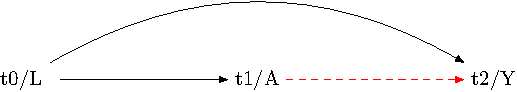
\includegraphics[width=0.8\textwidth,height=\textheight]{causal-dags_files/figure-pdf/fig-dag-common-cause-1.pdf}

}

\caption{\label{fig-dag-common-cause}Counfounding by a common cause. The
dashed path indicates bias arising from the open backdoor path from A to
Y.}

\end{figure}%

\subsubsection{Advice: attend to the temporal order of all measured
variables}\label{advice-attend-to-the-temporal-order-of-all-measured-variables}

Addressing confounding by a common cause involves its adjustment. This
adjustment effectively closes the backdoor path from the exposure to the
outcome. Equivalently, conditioning on \(L\) d-separates \(A\) and
\(Y\). Common adjustment methods include regression, matching, inverse
probability of treatment weighting, and G-methods (covered in
(\citeproc{ref-hernuxe1n2023}{Hernán and Robins 2023})).
Figure~\ref{fig-dag-common-cause-solution} clarifies that any confounder
that is a common cause of both \(A\) and \(Y\) must precede \(A\) (and
hence \(Y\)), since effects follow their causes chronologically.

After we have time-indexing the nodes on the graph it becomes evident
that \textbf{control of confounding generally requires time-series data
repeatedly measured on the units for which causal inferences apply.} Our
causal diagram is a circuit breaker that casts doubt on attempts for
causal inference in settings where researchers lack time series data.

\begin{figure}

\centering{

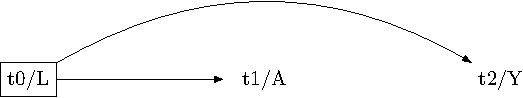
\includegraphics[width=0.8\textwidth,height=\textheight]{causal-dags_files/figure-pdf/fig-dag-common-cause-solution-1.pdf}

}

\caption{\label{fig-dag-common-cause-solution}Solution: adjust for
pre-exposure confounder. The implication: obtain time series data to
ensure the confounder occurs before the exposure.}

\end{figure}%

\subsubsection{2. Confounding by collider stratification (conditioning
on a common
effect)}\label{confounding-by-collider-stratification-conditioning-on-a-common-effect}

Conditioning on a common effect occurs when a variable \(L\) is affected
by the treatment \(A\) and an outcome \(Y\).

Suppose \(A\) and \(Y\) are initially independent, such that
\(A \coprod Y(a)\). Conditioning on the joint effect \(L\) opens a
backdoor path between \(A\) and \(Y\), potentially inducing a non-causal
association. This occurs because \(L\) can provide information about
both \(A\) and \(Y\).

To clarify, let \(A\) denote the level of belief in Big Gods (with
higher values indicating stronger belief), \(Y\) denote social
complexity, and \(L\) denote economic trade. Suppose that belief in Big
Gods and social complexity were not causally linked. That is, if we were
to intervene to foster such beliefs, this intervention would not itself
affect social complexity. However, suppose beliefs in Big Gods and
social complexity separately influence levels of economic trade (\(L\)).
Now suppose we were to condition on economic trade without attending to
temporal order -- perhaps because time series data are not available. In
that case, we might find a statistical association between belief in Big
Gods and social complexity without a causal association.\footnote{To
  clarify, denote the observed associations as follows:}

\begin{itemize}
\tightlist
\item
  \(P(A)\): Distribution of beliefs in Big Gods
\item
  \(P(Y)\): Distribution of social complexity
\item
  \(P(L)\): Distribution of economic trade
\end{itemize}

Without conditioning on \(L\), if \(A\) and \(Y\) are independent, we
have: \[P(A, Y) = P(A)P(Y)\]

However, if we condition on \(L\) (which is a common effect of both
\(A\) and \(Y\)), we have:

\begin{verbatim}
$$P(A, Y | L) \neq P(A | L)P(Y | L)$$
\end{verbatim}

Once conditioned on, the common effect \(L\) creates an association
between \(A\) and \(Y\) that is not causal. This association in the data
can mislead us into believing there is a direct link between beliefs in
Big Gods and social complexity, even without such a link. If we were to
only observed \(A\), \(Y\), and \(L\) in cross-sectional data, we might
erroneously conclude \(A \to Y\).

When \(A\) and \(Y\) are independent, the joint probability of \(A\) and
\(Y\) is equal to the product of their individual probabilities:
\(P(A, Y) = P(A)P(Y)\). However, when we condition on \(L\), the joint
probability of \(A\) and \(Y\) given \(L\) is not necessarily equal to
the product of the individual probabilities of \(A\) and \(Y\) given
\(L\), hence the inequality \(P(A, Y | L) \neq P(A | L)P(Y | L)\).

\begin{figure}

\centering{

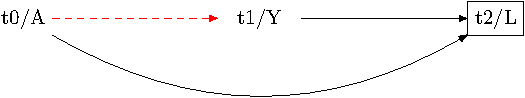
\includegraphics[width=0.8\textwidth,height=\textheight]{causal-dags_files/figure-pdf/fig-dag-common-effect-1.pdf}

}

\caption{\label{fig-dag-common-effect}Confounding by conditioning on a
collider. The dashed red path indicates bias from the open backdoor path
from A to Y.}

\end{figure}%

\subsubsection{Advice: attend to the temporal order of all measured
variables}\label{advice-attend-to-the-temporal-order-of-all-measured-variables-1}

To address the problem of conditioning on a common effect, we should
\emph{generally} ensure that:

\begin{enumerate}
\def\labelenumi{\arabic{enumi}.}
\tightlist
\item
  all confounders \(L\) that are common causes of the exposure \(A\) and
  the outcome \(Y\) are measured before \(A\) has occurred, and
\item
  \(A\) is measured before \(Y\) has occurred.
\end{enumerate}

If such temporal order is preserved, \(L\) cannot be an effect of \(A\),
and thus neither of \(Y\).\footnote{This rule is not absolute. As
  indicated in Figure~\ref{fig-dag-descendent-solution}, it may be
  helpful in certain circumstances to condition on a confounder that
  occurs \emph{after} the outcome has occurred.} In the example just
described for beliefs and social complexity, such assurance typically
requires time-series data with accurate measurements. Also required is a
sufficiently large sample of cultures that transition in religious
beliefs, with measurements of social complexity before and after.
Moreover, the cultures in the dataset would need to be independent of
each other.\footnote{The independence of cultural units was at the
  centre of the study of comparative urban archaeology from the late
  19th (\citeproc{ref-decoulanges1903}{De Coulanges 1903}) through the
  late 20th century (\citeproc{ref-wheatley1971}{Wheatley 1971}).
  Despite attention to this problem in recent work (e.g.
  (\citeproc{ref-watts2016}{Watts \emph{et al.} 2016})), there is
  arguably a greater head-room for understanding the need for
  conditional independence of cultures in recent cultural evolutionary
  studies. Again, attending to the temporal order of events is
  essential.}

\begin{figure}

\centering{

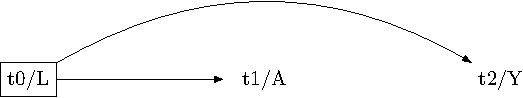
\includegraphics[width=0.8\textwidth,height=\textheight]{causal-dags_files/figure-pdf/fig-dag-common-effect-solution-1.pdf}

}

\caption{\label{fig-dag-common-effect-solution}Solution: time idexing of
confounders helps to avoid collider bias and maintain d-separation. The
graph makes the imperative clear: we must collect time series data with
confounders measured before the exposure, and that we must likewise
measure the exposure before the outcome, with data collected
repeatitively on the same units.}

\end{figure}%

\subsubsection{M-bias: conditioning on a collider that occurs before the
exposure may introduce
bias}\label{m-bias-conditioning-on-a-collider-that-occurs-before-the-exposure-may-introduce-bias}

Typically, indicators for confounders should be included only if they
are known to be measured before their exposures - with notable
exceptions described below in fig-dag-descendent-solution-2 and .

However, researchers should also be cautious about over-conditioning on
pre-exposure variables that are not associated with both the exposure
and confounder, as doing so can induce confounding. As shown in
Figure~\ref{fig-m-bias}, collider stratification may arise even if \(L\)
occurs before \(A\). This happens when \(L\) does not affect \(A\) or
\(Y\), but may be the descendent of an unmeasured variable that affects
\(A\) and another unmeasured variable that also affects \(Y\).
Conditioning on \(L\) in this scenario evokes ``M-bias.'' If \(L\) is
not a common cause of \(A\) and \(Y\), or the effect of a shared common
cause, \(L\) should not be included in a causal model.
Figure~\ref{fig-m-bias} presents a case in which \(A \coprod Y(a)\) but
\(A \cancel{\coprod} Y(a)| L\). M-bias is another example of collider
stratification bias (see: (\citeproc{ref-cole2010}{Cole \emph{et al.}
2010})).\footnote{Note, when we draw a chronologically ordered path from
  left to right the M shape for which ``M-bias'' takes its name changes
  to an E shape We shall avoid proliferating jargon and retain the term
  ``M bias.''}

\begin{figure}

\centering{

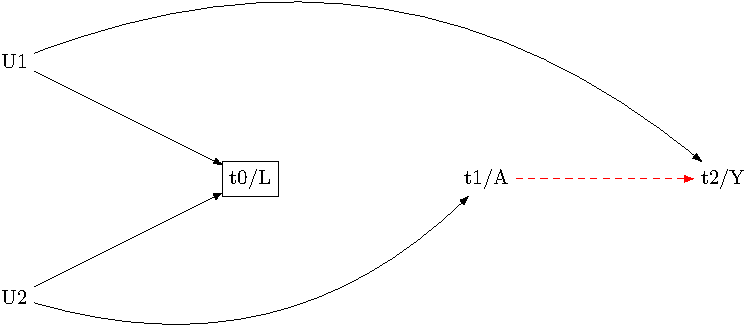
\includegraphics[width=0.8\textwidth,height=\textheight]{causal-dags_files/figure-pdf/fig-m-bias-1.pdf}

}

\caption{\label{fig-m-bias}M-bias: confounding control by including
previous outcome measures. The dashed red path indicates bias from the
open backdoor path from A to Y by conditioning on pre-exposure variable
L. The solution: do not condition on L. The graph makes it evident that
conditioning on variables measured before the exposure is not sufficient
to prevent confounding.}

\end{figure}%

\subsubsection{Advice: adopt the modified disjunctive cause criterion
for confounding
control}\label{advice-adopt-the-modified-disjunctive-cause-criterion-for-confounding-control}

Again, the modified disjunctive cause criterion will satisfy the
backdoor criterion in all cases and reduce bias where this criterion
cannot be fully satisfied:

\begin{enumerate}
\def\labelenumi{\alph{enumi}.}
\tightlist
\item
  Control for any variable that causes the exposure, the outcome, or
  both.
\item
  Control for any proxy for an unmeasured variable that is a shared
  cause of both exposure and outcome.
\item
  Define an instrumental variable as a variable associated with the
  exposure but does not influence the outcome independently, except
  through the exposure. Exclude any instrumental variable that is not a
  proxy for an unmeasured confounder from the confounder set (see:
  VanderWeele \emph{et al.} (\citeproc{ref-vanderweele2020}{2020}) page
  441, (\citeproc{ref-vanderweele2019}{VanderWeele 2019}))
\end{enumerate}

Of course, the difficulty is in determining which variables belong to a
confounder set. Specialist knowledge can facilitate this task. However,
the data alone typically do not settle this question. (For exceptions
see: bulbulia2021).

\subsubsection{3. Mediator bias}\label{mediator-bias}

Conditioning on a mediator -- a variable that lies along the causal
pathway between the treatment and the outcome -- can distort the total
effect of the treatment on the outcome and potentially introduce bias.
To illustrate this, consider ``beliefs in Big Gods'' as the treatment
(\(A\)), ``social complexity'' as the outcome (\(Y\)), and ``economic
trade'' as the mediator (\(L\)).

In this scenario, the belief in Big Gods (\(A\)) has a direct impact on
economic trade (\(L\)), which subsequently influences social complexity
(\(Y\)). If we condition on economic trade (\(L\)), we could bias our
estimates of the overall effect of beliefs in Big Gods (\(A\)) on social
complexity (\(Y\)). This bias happens because conditioning on \(L\) can
downplay the direct effect of \(A\) on \(Y\), as it blocks the indirect
path through \(L\). This problem, known as mediator bias, is illustrated
in Figure~\ref{fig-dag-mediator}.

We might think that conditioning on a mediator does not introduce bias
under a null hypothesis (\(A\) does not cause \(Y\)), however, this is
not the case. Consider a situation where \(L\) is a common effect of the
exposure \(A\) and an unmeasured variable \(U\) linked to the outcome
\(Y\). In this scenario, including \(L\) may amplify the association
between \(A\) and \(Y\), even if \(A\) is not associated with \(Y\) and
\(U\) does not cause \(A\). This scenario is represented in
Figure~\ref{fig-dag-descendent}.

So, unless one is explicitly investigating mediation analysis, it is
usually not advisable to condition on a post-treatment variable. Again,
attending to chronology in the the spatial organisation of the graph
reveals an imperative for data collection: if we cannot ensure that
\(L\) is measured before \(A\), and if \(A\) may affect \(L\), including
\(L\) in our model could result in mediator bias. This scenario is
presented in Figure~\ref{fig-dag-descendent}.

\begin{figure}

\centering{

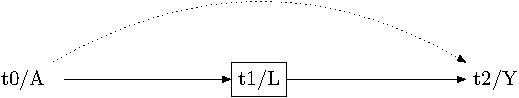
\includegraphics[width=0.8\textwidth,height=\textheight]{causal-dags_files/figure-pdf/fig-dag-mediator-1.pdf}

}

\caption{\label{fig-dag-mediator}Confounding by conditioning on a
mediator. The dashed black arrow indicates bias arising from partially
blocking the path between A and Y.}

\end{figure}%

\subsubsection{Advice: attend to the temporal order of all measured
variables}\label{advice-attend-to-the-temporal-order-of-all-measured-variables-2}

To mitigate the issue of mediator bias, particularly when focusing on
total effects, we should generally avoid conditioning on a mediator. We
avoid this problem by ensuring that \(L\) occurs before the treatment
\(A\) and the outcome \(Y\) (Note: a counter-example is presented in
Figure~\ref{fig-dag-descendent-solution-2}). Again, we discover the
importance of explicitly stating the temporal ordering of our
variables.\footnote{Note that if \(L\) were associated with \(Y\) and
  could not be caused by \(A\), conditioning on \(L\) would typically
  enhance the precision of the causal effect estimate of \(A \to Y\).
  This precision enhancement holds even if \(L\) occurs \emph{after}
  \(A\). However, the onus is on the researcher to show that the
  post-treatment factor cannot be a consequence of the exposure.}

\begin{figure}

\centering{

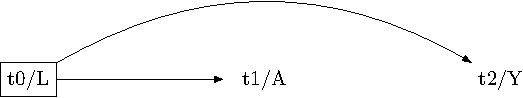
\includegraphics[width=0.8\textwidth,height=\textheight]{causal-dags_files/figure-pdf/fig-dag-mediator-solution-1.pdf}

}

\caption{\label{fig-dag-mediator-solution}Solution: do not condition on
a mediator. The implication: by ensuring temporal order in data
collection we diminish the probabilty of mistaking an effect of an
exposure for its confounder.}

\end{figure}%

\subsubsection{4. Conditioning on a descendant man induce
confounding}\label{conditioning-on-a-descendant-man-induce-confounding}

Say \(L\) is a cause of \(L^\prime\). According to Markov factorisation,
if we condition on \(L\), we partially condition on \(L^\prime\).

Consider how conditioning might imperil causal estimation. Suppose there
is a confounder \(L^\prime\) that is caused by an unobserved variable
\(U\), and is affected by the treatment \(A\). Suppose further that
\(U\) causes the outcome \(Y\). In this scenario, as described in
Figure~\ref{fig-dag-descendent}, conditioning on \(L^\prime\), which is
a descendant of \(A\) and \(U\), can lead to a spurious association
between \(A\) and \(Y\) through the path \(A \to L^\prime \to U \to Y\).

\begin{figure}

\centering{

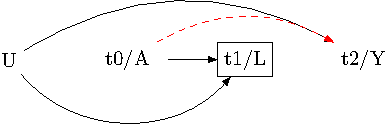
\includegraphics[width=0.8\textwidth,height=\textheight]{causal-dags_files/figure-pdf/fig-dag-descendent-1.pdf}

}

\caption{\label{fig-dag-descendent}Confounding by descent: the red
dashed path illustrates the introduction of bias by conditioning on the
descendant of a confounder that is affected by the exposure, thus
opening of a backdoor path between the exposure, A, and the outcome, Y.}

\end{figure}%

Again, the advice is evident from the chronology of the graph: we should
measure the (\(L^\prime\)) before the exposure (\(A\)). This strategy is
presented in Figure~\ref{fig-dag-descendent-solution}.

\begin{figure}

\centering{

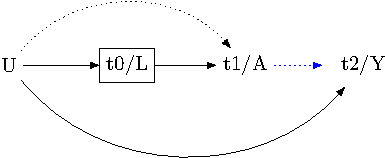
\includegraphics[width=0.8\textwidth,height=\textheight]{causal-dags_files/figure-pdf/fig-dag-descendent-solution-1.pdf}

}

\caption{\label{fig-dag-descendent-solution}Solution: again the graph
makes it clear that our data must ensure temporal order of the
measurements. By ensuring that L occurs before A confounding is
controlled. The figure also makes it evident that L need not affect Y to
be a confounder (i.e.~a member of a confounder set).}

\end{figure}%

\subsubsection{5. Conditioning on a descendent may reduce
confounding}\label{conditioning-on-a-descendent-may-reduce-confounding}

Next consider how we may use a post-treatment descendent to reduce bias.
Suppose an unmeasured confounder \(U\) affects \(A\), \(Y\), and
\(L^\prime\) as presented in, then adjusting for \(L^\prime\) may help
to reduce confounding caused by \(U\). This scenario is presented in
Figure~\ref{fig-dag-descendent-solution-2}. If we deploy the modified
disjunctive cause criterion for confounding control, we would ``include
as a covariate any proxy for an unmeasured variable that is a common
cause of both the exposure and the outcome''
(\citeproc{ref-vanderweele2019}{VanderWeele 2019}). We discover that
although \(L^\prime\) may occur \emph{after} the exposure, and indeed
occur \emph{after} the outcome, we may condition on it to reduce
confounding because it is a proxy for an unmeasured common cause of the
exposure and the confounder. \textbf{This example shows that employing a
rule that requires us to condition only on pre-exposure (and indeed
pre-outcome) variables would be hasty.} More generally,
fig-dag-descendent-solution-2 demonstrates the imperative for thinking
carefully about data collection. We cannot blindly apply alogrithic
rules about confounding control. Each problem must be approached anew.

\begin{figure}

\centering{

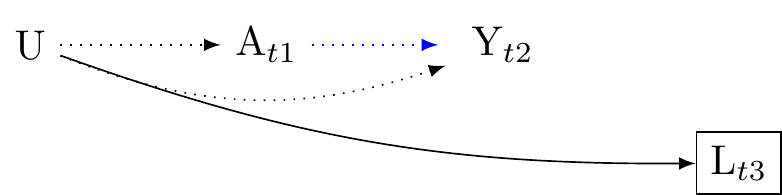
\includegraphics[width=0.8\textwidth,height=\textheight]{causal-dags_files/figure-pdf/fig-dag-descendent-solution-2-1.pdf}

}

\caption{\label{fig-dag-descendent-solution-2}Solution: conditioning on
a confounder that occurs after the exposure and the outcome might
address a problem of unmeasured confounding if the confounder is a
descendent of a prior common cause of the exposure and outcome. The
dotted paths denote that the effect of U on A and Y is partially
adjusted by conditioning on L', even though L' occurs after the outcome.
The paths are dotted to represent a reduction of bias by conditioning on
the post-outcome descendent of an unmeasured common cause of the
exposure and outcome. How might this work? Consider a genetic factor
that affects the exposure and the outcome early in life might be
measured by an indicator late that is expressed (and may be measured)
later in life. Adjusting for such an indicator would constitute an
example of post-outcome confounding control.}

\end{figure}%

\subsection{Part 3. Application of Causal Diagrams for Clarifying
Moderation (Interaction), Mediation, and Longitudinal
Growth.}\label{part-3.-application-of-causal-diagrams-for-clarifying-moderation-interaction-mediation-and-longitudinal-growth.}

\subsubsection{Case 1. Causal Interaction and Causal Effect
Modification: do not draw non-linear relationships such as
interactions}\label{case-1.-causal-interaction-and-causal-effect-modification-do-not-draw-non-linear-relationships-such-as-interactions}

Interactions are scientific interesting because we often wish to
understand for whom effects occur. How shall we depict interactions on a
graph? It is crucial to remember the primary function of causal diagrams
is to investigate confounding. Causal diagrams are not designed to
capture all facets of a phenomenon under investigation. We should not
attempt any unique visual trick to show additive and multiplicative
interaction. Moreover, we should include those nodes and paths as are
necessary to evaluate structural sources of bias. Causal graphs are
meant to be human read. They are not meant to be complete maps of causal
reality.

Misunderstandings arise about the role and function of causal diagrams
in application to interaction. Such misunderstandings typically stem
from a more profound confusion about the concept of interaction itself.
Given this deeper problem, it is worth clarifying the concept of causal
interaction as understood within the counterfactual causal framework.
Again, evaluating evidence for interaction is often essential for much
scientific research. However, we must distinguish between concepts of
causal interaction and concepts of causal effect modification because
these concepts address different causal questions.

\paragraph{\texorpdfstring{\textbf{Causal interaction as a double
exposure}}{Causal interaction as a double exposure}}\label{causal-interaction-as-a-double-exposure}

Causal interaction refers to the combined or separate (or non-existent)
effect of two exposures. Evidence for interaction on a given scale is
present when the effect of one exposure on an outcome depends on another
exposure's level. For instance, the impact of beliefs in Big Gods
(exposure A) on social complexity (outcome Y) might depend on a
culture's monumental architecture (exposure B), which could also
influence social complexity. Evidence of causal interaction on the
difference scale would be present if:

\[\bigg(\underbrace{\mathbb{E}[Y(1,1)]}_{\text{joint exposure}} - \underbrace{\mathbb{E}[Y(0,0)]}_{\text{neither exposed}}\bigg) - \bigg[ \bigg(\underbrace{\mathbb{E}[Y(1,0)]}_{\text{only A exposed}} - \underbrace{\mathbb{E}[Y(0,0)]}_{\text{neither exposed}}\bigg) + \bigg(\underbrace{\mathbb{E}[Y(0,1)]}_{\text{only B exposed}} - \underbrace{\mathbb{E}[Y(0,0)]}_{\text{neither exposed}} \bigg)\bigg] \neq 0 \]

This equation simplifies to

\[ \underbrace{\mathbb{E}[Y(1,1)]}_{\text{joint exposure}} - \underbrace{\mathbb{E}[Y(1,0)]}_{\text{only A exposed}} - \underbrace{\mathbb{E}[Y(0,1)]}_{\text{only B exposed}} + \underbrace{\mathbb{E}[Y(0,0)]}_{\text{neither exposed}} \neq 0 \]

If the above equation were to hold, the effect of exposure \(A\) on the
outcome \(Y\) would differ across levels of \(B\) or vice versa. Such a
difference would provide evidence for interaction.

If the value is positive, we say there is evidence for an additive
effect. If the value is less than zero, we say there is evidence for a
sub-additive effect. If the value is virtually zero, there is no
reliable evidence for interaction.\footnote{Note that causal effects of
  interactions often differ when measured on the ratio scale. This
  discrepency can have significant policy implications, see:
  (\citeproc{ref-vanderweele2014}{VanderWeele and Knol 2014}). Although
  beyond the scope of this article, when evaluating evidence for
  causality we must clarify the measure of effect in which we are
  interested (\citeproc{ref-hernuxe1n2004}{Hernán \emph{et al.} 2004};
  \citeproc{ref-tripepi2007}{Tripepi \emph{et al.} 2007}).}

Remember that causal diagrams are non-parametric. They do not directly
represent interactions. They are tools for addressing the identification
problem. Although a causal diagram can indicate an interaction's
presence by displaying two exposures jointly influencing an outcome, as
in Figure~\ref{fig-dag-interaction}, it does not directly represent the
interaction's nature or scale.

\begin{figure}

\centering{

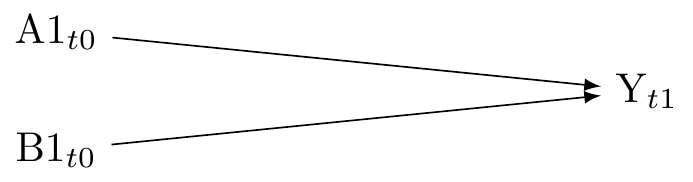
\includegraphics[width=0.6\textwidth,height=\textheight]{causal-dags_files/figure-pdf/fig-dag-interaction-1.pdf}

}

\caption{\label{fig-dag-interaction}Causal interaction: if two exposures
are causally independent of each other, we may wish to estimate their
individual and joint effects on Y, conditional on confounding control
strategy that blocks backdoor paths for bothe exposures (here, L1 and L2
are jointly required). where the counterfactual outcome is Y(a,b) and
there is evidence for additive or subadditive interaction if E{[}Y(1,1)
- Y(0,1) - Y(1,0) + Y(0,0){]} ≠ 0. If we cannot conceptualise B as a
variable upon which intervention can occur, then the interaction is
better conceived as effect modification (see next figure). Important: do
not attempt to draw a path into another path.}

\end{figure}%

\paragraph{\texorpdfstring{\textbf{Causal effect modification under a
single
exposure}}{Causal effect modification under a single exposure}}\label{causal-effect-modification-under-a-single-exposure}

With the analysis of effect modification, we aim to understand how an
exposure's effect varies, if at all, across levels of another variable,
an effect modifier.

Consider again the problem of estimating the causal effect of beliefs in
Big Gods on social complexity. Suppose this time we are interested in
the investigating whether this effect varies across early urban
civilisations in ancient China and South America. In this example
geography (China versus South America) is an ``effect modifier.'' Here,
we do not treat the effect modifier as an intervention. Rather, we wish
to investigate whether geography is a parameter that may alter the
exposure's effect on an outcome.

For clarity, consider comparing two exposure levels, represented as
\(A = a\) and \(A= a^*\). Further, assume that \(G\) represents two
levels of effect-modification, represented as \(g\) and \(g'\).

Then, the expected outcome when exposure is at level \(A=a\) among
individuals in group \(G=g\) is expressed

\[\hat{E}[Y(a)|G=g]\]

The expected outcome when exposure is at level \(A=a^*\) among
individuals in group \(G=g\) is expressed

\[\hat{E}[Y(a^*)|G=g]\]

The causal effect of shifting the exposure level from \(a^*\) to \(a\)
in group \(g\) is expressed

\[\hat{\delta}_g = \hat{\mathbb{E}}[Y(a)|G=g] - \hat{\mathbb{E}}[Y(a^*)|G=g]\]

Likewise, the causal effect of changing the exposure from \(a^*\) to
\(a\) in group \(g'\) is expressed.

\[\hat{\delta}_{g'} = \hat{\mathbb{E}}[Y(a)|G=g'] - \hat{\mathbb{E}}[Y(a^*)|G=g']\]

We compare the causal effect on the difference scale in these two groups
by computing

\[\hat{\gamma} = \hat{\delta}_g - \hat{\delta}_{g'}\]

The value of \(\hat{\gamma}\) quantifies how the effect of shifting the
exposure from \(a^*\) to \(a\) differs between groups \(g\) and \(g'\).

If \(\hat{\gamma}\neq 0\), then there is evidence for effect
modification. We may infer the exposure's effect varies by geography.

Again, remember that causal diagrams are non-parametric. More
fundamental, causal diagrams function to identify structural sources of
bias and to help researchers develop strategies for addressing such
bias. We should not draw an intersecting path or attempt other
visualisations to represent effect modification. Instead, we should draw
two edges into the exposure. This is depicted in
Figure~\ref{fig-dag-effect-modfication}.\footnote{For distinctions
  within varieties of effect modification relevant for strategies of
  confounding controul see (\citeproc{ref-vanderweele2007}{VanderWeele
  and Robins 2007}).}

\begin{figure}

\centering{

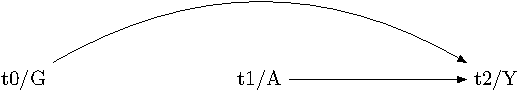
\includegraphics[width=0.8\textwidth,height=\textheight]{causal-dags_files/figure-pdf/fig-dag-effect-modfication-1.pdf}

}

\caption{\label{fig-dag-effect-modfication}A simple graph for
effect-modification in which there are no confounders. G is an effect
modifier of A on Y. We draw a box around G to indicate we are
conditioning on this variable.}

\end{figure}%

\subsubsection{Case 2: Causal mediation: causal diagrams reveal the
inadequacy of standard
approaches}\label{case-2-causal-mediation-causal-diagrams-reveal-the-inadequacy-of-standard-approaches}

The conditions necessary for causal mediation are stringent. I present
these conditions in the chronologically ordered causal diagram shown in
Figure~\ref{fig-dag-mediation-assumptions}. We will again consider
whether cultural beliefs in Big Gods affect social complexity. We now
ask whether this affect is mediated by political authority. The
assumptions required for asking causal mediation questions are as
follows

\begin{enumerate}
\def\labelenumi{\arabic{enumi}.}
\tightlist
\item
  \textbf{No unmeasured exposure-outcome confounder}
\end{enumerate}

This prerequisite is expressed: \(Y(a,m) \coprod A | L1\). Upon
controlling for the covariate set \(L1\), we must ensure that no
additional unmeasured confounders affect both the cultural beliefs in
Big Gods \(A\) and the social complexity \(Y\). For example, suppose our
study involves the effect of cultural beliefs in Big Gods (exposure) on
social complexity (outcome), and geographic location and historical
context define the covariates in \(L1\). In that case, we must assume
that accounting for \(L1\) d-separates \(A\) and \(Y\). The relevant
confounding path is depicted in brown in
Figure~\ref{fig-dag-mediation-assumptions}.

\begin{enumerate}
\def\labelenumi{\arabic{enumi}.}
\setcounter{enumi}{1}
\tightlist
\item
  \textbf{No unmeasured mediator-outcome confounder}
\end{enumerate}

This condition is expressed: \(Y(a,m) \coprod M | L2\). After
controlling for the covariate set \(L2\), we must ensure that no other
unmeasured confounders affect the political authority \(M\) and social
complexity \(Y\). For instance, if trade networks impact political
authority and social complexity, we must account for trade networks to
obstruct the unblocked path linking our mediator and outcome. Further,
we must assume the absence of any other confounders for the
mediator-outcome path. This confounding path is represented in blue in
Figure~\ref{fig-dag-mediation-assumptions}.

\begin{enumerate}
\def\labelenumi{\arabic{enumi}.}
\setcounter{enumi}{2}
\tightlist
\item
  \textbf{No unmeasured exposure-mediator confounder}
\end{enumerate}

This requirement is expressed: \(M(a) \coprod A | L3\). Upon controlling
for the covariate set \(L3\), we must ensure that no additional
unmeasured confounders affect both the cultural beliefs in Big Gods
\(A\) and political authority \(M\). For example, the capability to
construct large ritual theatres may influence the belief in Big Gods and
the level of political authority. If we have indicators for this
technology measured prior to the emergence of Big Gods (these indicators
being \(L3\)), we must assume that accounting for \(L3\) closes the
backdoor path between the exposure and the mediator. This confounding
path is shown in green in Figure~\ref{fig-dag-mediation-assumptions}.

\begin{enumerate}
\def\labelenumi{\arabic{enumi}.}
\setcounter{enumi}{3}
\tightlist
\item
  \textbf{No mediator-outcome confounder affected by the exposure}
\end{enumerate}

This requirement is expressed: \(Y(a,m) \coprod M(a^*) | L\). We must
ensure that no variables confounding the relationship between political
authority and social complexity in \(L2\) are themselves influenced by
the cultural beliefs in Big Gods (\(A\)). For instance, when studying
the effect of cultural beliefs in Big Gods (\(A\), the exposure) on
social complexity (\(Y\), the outcome) as mediated by political
authority (mediator), there can be no factors, such as trade networks
(\(L2\)), that influence both political authority and social complexity
and are affected by the belief in Big Gods. This confounding path is
shown in red in Figure~\ref{fig-dag-mediation-assumptions}. \textbf{Note
that the assumption of no exposure-induced confounding in the
mediator-outcome relationship is often a substantial obstacle for causal
mediation analysis.} If the exposure influences a confounder of the
mediator and outcome, we face a dilemma. Without accounting for this
confounder, the backdoor path between the mediator and the outcome
remains open. By accounting for it, however, we partially obstruct the
path between the exposure and the mediator, leading to bias.
Consequently, observed data cannot identify the natural direct and
indirect effects.

Notice again that the requirements for counterfactual data science are
more strict than for descriptive or predictive data science.

We have now considered how chronologically ordered causal diagrams
elucidate the conditions necessary for causal mediation
analysis.\footnote{An excellent resource both for understanding causal
  interaction and causal mediation is
  (\citeproc{ref-vanderweele2015}{VanderWeele 2015}).}

\begin{figure}

\centering{

\includegraphics[width=1\textwidth,height=\textheight]{causal-dags_files/figure-pdf/fig-dag-mediation-assumptions-1.pdf}

}

\caption{\label{fig-dag-mediation-assumptions}This causal diagram
illustrates the four fundamental assumptions needed for causal mediation
analysis. The first assumption pertains to the brown paths. It requires
the absence of an unmeasured exposure-outcome confounder, and assumes
that conditioning on L1 is sufficient for such confounding control. The
second assumption pertains to the blue paths. It requires the absence of
an unmeasured mediator-outcome confounder, and assumes that conditioning
on L2 is sufficient for such confounding control. The third assumption
pertains to the green paths. It requires the absence of an unmeasured
exposure-mediator confounder, and assumes that conditioning on L3 is
sufficient for such confounding control. The fourth and final assumption
pertains to the red paths. It requires the absence of an a
mediator-outcome confounder that is affected by the exposure, and
assumes that there is no path from the exposure to L2 to M. If the
exposure were to affect L2, then conditioning on L2 would block the
exposure's effect on the mediator, as indicated by dashed red path.
Causal diagrams not only clarify how different types of confounding bias
may converge (here mediation bias and confounder bias), but also reveal
the limitations of common methods such as structural equation models and
multilevel models for handling time-series data where the fourth
assumption fails -- that is, where there is treatment-confounder
feedback. Such feedback is common in time-series data, but not widely
understood. For example structural equation models and multi-level
models cannot address causal questions in the presence of such feedback,
but these models remain widely favoured.}

\end{figure}%

\subsubsection{Case 3: Confounder-Treatment Feedback: Longitudinal
``growth'' is not
causation}\label{case-3-confounder-treatment-feedback-longitudinal-growth-is-not-causation}

In our discussion of causal mediation, we consider how the effects of
two sequential exposures may combine to affect an outcome. We can
broaden this interest to consider the causal effects of multiple
sequential exposures. In such scenarios, causal diagrams arranged
chronologically can aid in clarifying the challenges and opportunities.

For example, consider temporally fixed multiple exposures. The
counterfactual outcomes may be denoted \(Y(a_{t1} ,a_{t2})\). There are
four counterfactual outcomes corresponding to the four fixed ``treatment
regimes:''

\begin{enumerate}
\def\labelenumi{\arabic{enumi}.}
\item
  \textbf{Always treat (Y(1,1))}
\item
  \textbf{Never treat (Y(0,0))}
\item
  \textbf{Treat once first (Y(1,0))}
\item
  \textbf{Treat once second (Y(0,1))}
\end{enumerate}

\begin{longtable}[]{@{}
  >{\raggedright\arraybackslash}p{(\columnwidth - 4\tabcolsep) * \real{0.1351}}
  >{\raggedright\arraybackslash}p{(\columnwidth - 4\tabcolsep) * \real{0.5405}}
  >{\raggedright\arraybackslash}p{(\columnwidth - 4\tabcolsep) * \real{0.3243}}@{}}
\caption{Table describes four fixed treatment regimes and six causal
contrasts in time series data where the exposure may
vary.}\label{tbl-regimes}\tabularnewline
\toprule\noalign{}
\begin{minipage}[b]{\linewidth}\raggedright
Type
\end{minipage} & \begin{minipage}[b]{\linewidth}\raggedright
Description
\end{minipage} & \begin{minipage}[b]{\linewidth}\raggedright
Counterfactual Outcome
\end{minipage} \\
\midrule\noalign{}
\endfirsthead
\toprule\noalign{}
\begin{minipage}[b]{\linewidth}\raggedright
Type
\end{minipage} & \begin{minipage}[b]{\linewidth}\raggedright
Description
\end{minipage} & \begin{minipage}[b]{\linewidth}\raggedright
Counterfactual Outcome
\end{minipage} \\
\midrule\noalign{}
\endhead
\bottomrule\noalign{}
\endlastfoot
Regime & Always treat & Y(1,1) \\
Regime & Never treat & Y(0,0) \\
Regime & Treat once first & Y(1,0) \\
Regime & Treat once second & Y(0,1) \\
Contrast & Always treat vs.~Never treat & E{[}Y(1,1) - Y(0,0){]} \\
Contrast & Always treat vs.~Treat once first & E{[}Y(1,1) - Y(1,0){]} \\
Contrast & Always treat vs.~Treat once second & E{[}Y(1,1) -
Y(0,1){]} \\
Contrast & Never treat vs.~Treat once first & E{[}Y(0,0) - Y(1,0){]} \\
Contrast & Never treat vs.~Treat once second & E{[}Y(0,0) - Y(0,1){]} \\
Contrast & Treat once first vs.~Treat once second & E{[}Y(1,0) -
Y(0,1){]} \\
\end{longtable}

There are six causal contrasts that we might compute for the four fixed
regimes, presented in Table~\ref{tbl-regimes}.\footnote{We compute the
  number of possible combinations of contrasts by
  \(C(n, r) = \frac{n!}{(n-r)! \cdot r!}\)}

Not that treatment assignments might be sensibly approached as a
function of the previous outcome. For example, we might \textbf{treat
once first} and then decide whether to treat again depending on the
outcome of the initial treatment. This aspect is known as ``time-varying
treatment regimes.''

Bear in mind that to estimate the ``effect'' of a time-varying treatment
regime, we are obligated to make comparisons between the relevant
counterfactual quantities. As mediation can introduce the possibility of
time-varying confounding (condition 4: the exposure must not impact the
confounders of the mediator/outcome path), the same holds true for all
sequential time-varying treatments. However, unlike conventional causal
mediation analysis, it might be necessary to consider the sequence of
treatment regimes over an indefinitely long period.

Chronologically organised causal diagrams are useful for highlighting
problems with traditional multi-level regression analysis and structural
equation modelling.

For example, we might be interested in whether belief in Big Gods
affects social complexity. Consider estimating a fixed treatment regime
first. Suppose we have a well-defined concept of Big Gods and social
complexity as well as excellent measurements for both over time. In that
case, we might want to assess the effects of beliefs in Big Gods on
social complexity, say, two centuries after the beliefs were introduced.

The fixed treatment strategies are: ``always believe in Big Gods''
versus ``never believe in Big Gods'' on the level of social complexity.
Refer to Figure~\ref{fig-dag-9}. Here, \(A_{tx}\) represents the
cultural belief in Big Gods at time \(tx\), and \(Y_{tx}\) is the
outcome, social complexity, at time \(x\). Imagine that economic trade,
denoted as \(L_{tx}\), is a time-varying confounder. Suppose its effect
changes over time, which in turns affects the factors that influence
economic trade. To complete our causal diagram, we might include an
unmeasured confounder \(U\), such as oral traditions, which could
influence both the belief in Big Gods and social complexity.

Consider a scenario where we can reasonably infer that the level of
economic trade at time \(0\), represented as \(L_{t0}\), impacts beliefs
in ``Big Gods'' at time \(1\), denoted as \(A_{t1}\). In this case, we
would draw an arrow from \(L_{t0}\) to \(A_{t1}\). Conversely, if we
assume that belief in ``Big Gods,'' \(A_{t1}\), influences the future
level of economic trade, \(L_{t2}\), then an arrow should be added from
\(A_{t1}\) to \(L_{t2}\). This causal diagram illustrates a feedback
process between the time-varying exposure \(A\) and the time-varying
confounder \(L\). Figure~\ref{fig-dag-9}. displays exposure-confounder
feedback. In practical settings, the diagram could contain more arrows.
However, the intention here is to use the minimal number of arrows
needed to demonstrate the issue of exposure-confounder feedback. As a
guideline, we should avoid overcomplicating our causal diagrams and aim
to include only the essential details necessary for assessing the
identification problem.

What would happen if we were to condition on the time-varying confounder
\(L_{t3}\)? Two things would occur. First, we would block all the
backdoor paths between the exposure \(A_{t2}\) and the outcome. We need
to block those paths to eliminate confounding. Therefore, conditioning
on the time-varying confounding is essential. However, paths that were
previously blocked would close. For example, the path
\(A_{t1}, L_{t2}, U, Y_{t4}\), that was previously closed would be
opened because the time-varying confounder is the common effect of
\(A_{t1}\) and \(U\). Conditioning, then, opens the path
\(A_{t1}, L_{t2}, U, Y_{t4}\). Therefore we must avoid conditioning on
the time-varying confounder. It would seem then that if we were to
condition on a confounder that is affected by the prior exposure, we are
``damned if we do'' and ``dammed if we do not.''

\begin{figure}

\centering{

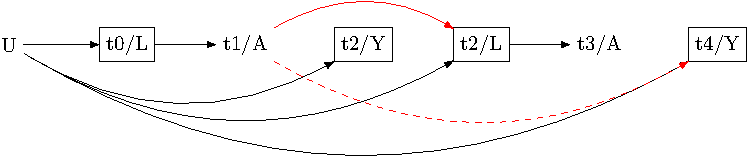
\includegraphics[width=1\textwidth,height=\textheight]{causal-dags_files/figure-pdf/fig-dag-9-1.pdf}

}

\caption{\label{fig-dag-9}Exposure confounder feedback is a problem for
time-series models. If we do not condition on L\_t2, a backdoor path is
open from A\_t3 to Y\_t4. However, if conditioning on L\_t2 introduces
collider bias, opening a path, coloured in red, between A\_t2 and Y\_t4.
Here, we may not use conventional methods to estimate the effects of
multiple exposures. Instead, at best, we may obtain controlled effects
using G-methods. Multi-level models will not eliminate bias (!).
However, outside of epidemiology, G-methods are presently rarely used.}

\end{figure}%

A similar problem arises when a time-varying exposure and time-varying
confounder share a common cause. This problem arises even without the
exposure affecting the confounder. The problem is presented in
Figure~\ref{fig-dag-time-vary-common-cause-A1-l1}.

\begin{figure}

\centering{

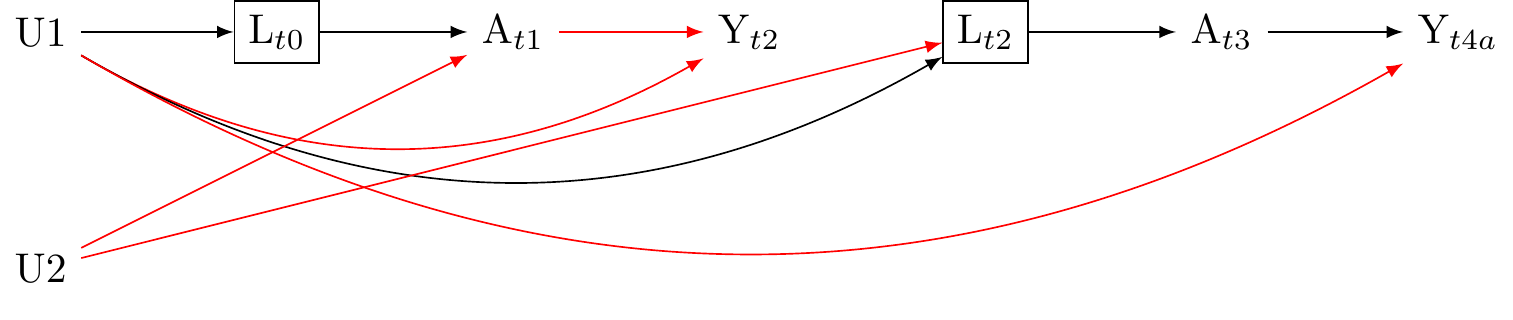
\includegraphics[width=1\textwidth,height=\textheight]{causal-dags_files/figure-pdf/fig-dag-time-vary-common-cause-A1-l1-1.pdf}

}

\caption{\label{fig-dag-time-vary-common-cause-A1-l1}Exposure confounder
feedback is a problem for time-series models. Here, the problem arises
from an unmeasured variable (U\_2) that affects both the exposure A at
time 1 and the cofounder L at time 2. The red paths show the open
backdoor path when we condition on the L at time 2. Again, we cannot
infer causal effects in such scenarios by using regression-based
methods. In this setting, to address causal questions, we require
G-methods.}

\end{figure}%

The potential for confounding increases when the exposure \(A_{t1}\)
affects the outcome \(Y_{t4}\). For example, since \(L_{t2}\) is on the
path from \(A_{t1}\) to \(Y_{t4}\), conditioning on \(L_{t2}\) partially
blocks the relation between the exposure and the outcome, triggering
collider stratification bias and mediator bias. However, to close the
open backdoor path from \(L_{t2}\) to \(Y_{t4}\), it becomes necessary
to condition on \(L_{t2}\). Paradoxically, we have just stated that
conditioning should be avoided! This broader dilemma of
exposure-confounder feedback is thoroughly explored in
(\citeproc{ref-hernuxe1n2023}{Hernán and Robins 2023}). Treatment
confounder feedback is particularly challenging for evolutionary human
science, yet its handling is beyond the capabilities of conventional
regression-based methods, including multi-level models
(\citeproc{ref-hernuxe1n2006}{Hernán and Robins 2006};
\citeproc{ref-robins1986}{Robins 1986}; \citeproc{ref-robins1999}{Robins
\emph{et al.} 1999}). As mentioned previously, G-methods encompass
models appropriate for investigating the causal effects of both
time-fixed and time-varying exposures
(\citeproc{ref-chatton2020}{Chatton \emph{et al.} 2020};
\citeproc{ref-hernuxe1n2006}{Hernán and Robins 2006};
\citeproc{ref-naimi2017}{Naimi \emph{et al.} 2017}). Despite significant
recent advancements in the health sciences
(\citeproc{ref-breskin2020}{Breskin \emph{et al.} 2020};
\citeproc{ref-duxedaz2021}{Díaz \emph{et al.} 2021};
\citeproc{ref-williams2021}{Williams and Díaz 2021}), these methods have
not been widely embraced in the field of human evolutionary sciences
\footnote{It is worth noting that the identification of controlled
  effect estimates can be enhanced by graphical methods such as ``Single
  World Intervention Graphs'' (SWIGs), which represent counterfactual
  outcomes in the diagrams. However, SWIGs are more accurately
  considered templates rather than causal diagrams in their general
  form. The use of SWIGs extends beyond the scope of this tutorial. For
  more information, see Richardson and Robins
  (\citeproc{ref-richardson2013}{2013}).}

\subsubsection{Summary}\label{summary}

To consistently estimate causal effects, we must contrast the world as
it has been with the world as it might have been. For many questions in
evolutionary human science, we have seen that confounder-treatment
feedback leads to intractable causal identification problems. We have
also seen that causal diagrams are helpful in clarifying these problems.
Many self-inflicted injuries, such as mediator bias and
post-stratification bias, could be avoided if confounders were measured
prior to the exposures. Chronologically ordered causal diagrams aim to
make this basis transparent. They function as circuit-breakers that may
protect us from blowing up our causal inferences. More constructively,
temporal order in the graph focusses attention on imperatives for data
collection, offering guidance and hope.

\subsection{Conclusions}\label{conclusions}

Chronologically ordered causal diagrams provide significant enrichment
to causal inference endeavours. Their utility is not limited to just
modelling; they serve as valuable guides for data collection, too. When
used judiciously, within the frameworks of counterfactual data science
that support causal inference, causal diagrams can substantially enhance
the pursuit of accurate and robust causal understanding. Here is a
summary of advice.

\subsubsection{Tips}\label{tips}

\begin{enumerate}
\def\labelenumi{\arabic{enumi}.}
\item
  Clearly define all nodes on the graph. Ambiguity leads to confusion.
\item
  Simplify the graph by combining nodes where this is possible. Keep
  only those nodes and edges that are essential for clarifying the
  identification problem at hand. Avoid clutter.
\item
  Define any novel convention in your diagram explicitly. Do not assume
  familiarity.
\item
  Ensure acyclicity in the graph. This guarantees that a node cannot be
  its own ancestor, thereby eliminating circular paths.
\item
  Maintain chronological order spatially. Arrange nodes in temporal
  sequence, usually from left to right or top to bottom. Although it is
  not necessary to draw the sequence to scale, the order of events
  should be clear from the layout.
\item
  Time-stamp nodes. Causation happens over time; reflect this visually
  in the diagrams.
\item
  Be pragmatic. Use the \emph{modified disjunctive cause criterion} to
  minimise or possibly eliminate bias. As we discussed in Part 2, this
  criterion identifies a variable as part of a confounder set if it can
  reduce bias stemming from confounding, even if bias cannot be
  eliminated. Using this criterion will typically reduce your reliance
  on sensitivity analyses.
\item
  Draw nodes for unmeasured confounding where it aids confounding
  control strategies. Assume unmeasured confounding always exists,
  whether depicted on the graph or not. This assumption reveals the
  importance of sensitivity analyses when estimating causal effects.
\item
  Illustrate nodes for post-treatment selection. This facilitates
  understanding of potential sources of selection bias.
\item
  Apply a two-step strategy: Initially, isolate confounding bias and
  selection bias, then contemplate measurement bias using a secondary
  graph. This approach will foster clarity.\footnote{See Hernán and
    Robins (\citeproc{ref-hernuxe1n2023}{2023}) p.125}
\end{enumerate}

\begin{enumerate}
\def\labelenumi{\arabic{enumi}.}
\setcounter{enumi}{10}
\item
  Expand graphs to clarify relevant bias structures if mediation or
  interaction is of interest. However, do not attempt to draw non-linear
  associations between variables.
\item
  Remember, causal diagrams are qualitative tools encoding assumptions
  about causal ancestries. They are compasses, not comprehensive
  atlases.
\end{enumerate}

\subsubsection{Pitfalls}\label{pitfalls}

\begin{enumerate}
\def\labelenumi{\arabic{enumi}.}
\item
  Misunderstanding the role of causal diagrams within the framework of
  counter-factual data science.
\item
  The causal diagram contains variables without time indices. This
  omission may suggest that the researcher has not adequately considered
  the timing of events.
\item
  The graph has excessive nodes. No effort has been made to simplify the
  model by retaining only those nodes and edges essential for clarifying
  the identification problem.
\item
  The study is an experiment, but arrows are leading into the
  manipulation, revealing confusion.
\item
  Bias is incorrectly described. The exposure and outcome are
  d-separated, yet bias is claimed. This indicates a misunderstanding;
  the bias probably relates to generalisability or transportability, not
  to confounding.
\item
  Overlooking the representation of selection bias on the graph,
  particularly post-exposure selection bias from attrition or
  missingness.
\item
  Neglecting to use causal diagrams during the design phase of research
  before data collection.
\item
  Ignoring structural assumptions in classical measurement theory, such
  as in latent factor models, and blindly using construct measures
  derived from factor analysis.
\item
  Trying to represent interactions and non-linear dynamics on a causal
  diagram, which can lead to confusion about their purposes.
\item
  Failing to realise that structural equation models are not structural
  models. They are tools for statistical analysis, better termed as
  ``correlational equation models.'' Coefficients from these models
  often lack causal interpretations.
\item
  Neglecting the fact that conventional models such as multi-level (or
  mixed effects) models are unsuitable when treatment-confounder
  feedback is present. Illustrating treatment-confounder feedback on a
  graph underscores this point.\footnote{G-methods are appropriate for
    causal estimation in dynamic longitudinal settings. Their
    effectiveness notwithstanding, many evolutionary human scientists
    have not adopted them.{[}\^{}g-methods-cites{]} For good
    introductions see: Hernán and Robins
    (\citeproc{ref-hernuxe1n2023}{2023}) Díaz \emph{et al.}
    (\citeproc{ref-duxedaz2021}{2021}) VanderWeele
    (\citeproc{ref-vanderweele2015}{2015}) Hoffman \emph{et al.}
    (\citeproc{ref-hoffman2022}{2022}) Hoffman \emph{et al.}
    (\citeproc{ref-hoffman2023}{2023}) Chatton \emph{et al.}
    (\citeproc{ref-chatton2020}{2020}) Shiba and Kawahara
    (\citeproc{ref-shiba2021}{2021}) Sjölander
    (\citeproc{ref-sjuxf6lander2016}{2016}) Breskin \emph{et al.}
    (\citeproc{ref-breskin2020}{2020}) VanderWeele
    (\citeproc{ref-vanderweele2009a}{2009b}) Vansteelandt \emph{et al.}
    (\citeproc{ref-vansteelandt2012}{2012}) Shi \emph{et al.}
    (\citeproc{ref-shi2021}{2021}).)}
\end{enumerate}

\begin{enumerate}
\def\labelenumi{\arabic{enumi}.}
\setcounter{enumi}{11}
\tightlist
\item
  Failing to recognise that simple models work for time series data with
  three measurement intervals. A multi-level regression does not make
  sense for the three-wave panel design described in Part 3.
\end{enumerate}

\subsubsection{Concluding remarks}\label{concluding-remarks}

In causal analysis, the passage of time is not just another variable but
the stage on which the entire causal play unfolds. Time-ordered causal
diagrams articulate this temporal structure, revealing the necessity for
collecting time-series data in our quest to answer our causal questions.

This need places new demands on our research designs, funding
mechanisms, and the very rhythm of scientific investigation. Rather than
continuing in the high-throughput, assembly-line model of research,
where rapid publication may sometimes come at the expense of depth and
precision, we must pivot towards an approach that nurtures the careful
and extended collection of data over time.

The pace of scientific progress in the human sciences of causal
inference hinges on this transformation. Our challenge is not merely
methodological but institutional, requiring a shift in our scientific
culture towards one that values the slow but essential work of building
rich, time-resolved data sets.

\newpage{}

\subsection{Funding}\label{funding}

This work is supported by a grant from the Templeton Religion Trust
(TRT0418). JB received support from the Max Planck Institute for the
Science of Human History. The funders had no role in preparing the
manuscript or the decision to publish it.

\subsection{References}\label{references}

\newpage{}

\subsection{Appendix 1: The difficulty of satisfying the three
fundamental assumptions of causal inference when asking causal questions
of
history}\label{appendix-1-the-difficulty-of-satisfying-the-three-fundamental-assumptions-of-causal-inference-when-asking-causal-questions-of-history}

Consider the Protestant Reformation of the 16th century, which initiated
religious change throughout much of Europe. Historians have argued that
Protestantism caused social, cultural, and economic changes in those
societies where it took hold (see: (\citeproc{ref-basten2013}{Basten and
Betz 2013}; \citeproc{ref-swanson1967}{Swanson 1967};
\citeproc{ref-swanson1971}{Swanson 1971}; \citeproc{ref-weber1905}{Weber
1905}, \citeproc{ref-weber1993}{1993}), for an overview see:
(\citeproc{ref-becker2016}{Becker \emph{et al.} 2016})).

Suppose we are interested in estimating the ``Average Treatment Effect''
of the Protestant Reformation. Let \(A = a^*\) denote the adoption of
Protestantism. We compare this effect with that of remaining Catholic,
represented as \(A = a\). We assume that both the concepts of ``adopting
Protestantism'' and of ``economic development'' are well-defined
(e.g.~GDP +1 century after a country has a Protestant majority
contrasted with remaining Catholic). The causal effect for any
individual country is \(Y_i(a^*) - Y_i(a)\). Although we cannot identify
this effect, if the basic assumptions of causal inference are met, we
can estimate the average or marginal effect as

\[
\frac{1}{n} \sum_i^{n} \left[ Y_i(a^*) - Y_i(a) \right]
\]

which, conditioning the confounding effects of \(L\) gives us

\[ATE_{\textnormal{economic~development}} = \mathbb{E}[Y(\textnormal{Became~Protestant}|L) - Y(\textnormal{Remained~Catholic}|L)]\]

When asking causal questions about the economic effect of adopting
Protestantism versus remaining Catholic, there are indeed several
challenges that arise in relation to the three fundamental assumptions
required for causal inference.

\textbf{Causal Consistency}: requires the outcome under each level of
exposure is well-defined. In this context, defining what ``adopting
Protestantism'' and ``remaining Catholic'' mean may present challenges.
The practices and beliefs associated with each religion might vary
significantly across countries and time periods, and it may be difficult
to create a consistent, well-defined exposure. Furthermore, the outcome
- economic development - may also be challenging to measure consistently
across different countries and time periods.

There is undoubtedly considerable heterogeneity in the ``Protestant
exposure.'' In England, Protestantism was closely tied to the monarchy
(\citeproc{ref-collinson2007}{Collinson 2007}). In Germany, Martin
Luther's teachings emphasised individual faith in scripture, which, it
has been claimed, supported economic development by promoting literacy
(\citeproc{ref-gawthrop1984}{Gawthrop and Strauss 1984}). In England,
King Henry VIII abolished Catholicism
(\citeproc{ref-collinson2007}{Collinson 2007}). The Reformation, then,
occurred differently in different places. The exposure needs to be
better-defined.

There is also ample scope for interference: 16th century societies were
interconnected through trade, diplomacy, and warfare. Thus, the
religious decisions of one society were unlikely to have been
independent from those of other societies.

\textbf{Exchangeability}: requires that given the confounders, the
potential outcomes are independent of the treatment assignment. It might
be difficult to account for all possible confounders in this context.
For example, historical, political, social, and geographical factors
could influence both a country's religious affiliations and its economic
development. If these factors are not properly controlled, it could lead
to confounding bias.

\textbf{Positivity}: requires that there is a non-zero probability of
every level of exposure for every strata of confounders. If we consider
various confounding factors such as geographical location, historical
events, or political circumstances, some countries might only ever have
the possibility of either remaining Catholic or becoming Protestant, but
not both. For example, it is unclear under which conditions 16th century
Spain could have been randomly assigned to Protestantism
(\citeproc{ref-nalle1987}{Nalle 1987}).

Perhaps a more credible measure of effect in the region of our interests
is the Average Treatment Effect in the Treated (ATT) expressed

\[ATT_{\textnormal{economic~development}} = \mathbb{E}[(Y(a*)- Y(a))|A = a*,L]\]

Here, the ATT defines the expected difference in economic success for
cultures that became Protestant compared with the expected economic
success if those cultures had not become Protestant, conditional on
measured confounders \(L\), among the exposed (\(A = a^*\)). To estimate
this contrast, our models would need to match Protestant cultures with
comparable Catholic cultures effectively. By estimating the ATT, we
would avoid the assumption of non-deterministic positivity for the
untreated. However, whether matching is conceptually plausible remains
debatable. Ostensibly, it would seem that assigning a religion to a
culture a religion is not as easy as administering a pill
(\citeproc{ref-watts2018}{Watts \emph{et al.} 2018}).

\subsection{Appendix 2: Review of VanderWeele's theory of causal
inference under multiple versions of
treatment}\label{appendix-2-review-of-vanderweeles-theory-of-causal-inference-under-multiple-versions-of-treatment}

We denote an average causal effect as the change in the expected
potential outcomes when all units receive one level of treatment
compared to another.

Let \(\delta\) denote the causal estimand on the difference scale
\((\mathbb{E}[Y^1 - Y^0])\). The causal effect identification can be
expressed as:

\[ \delta = \sum_l \left( \mathbb{E}[Y|A=a,l] - \mathbb{E}[Y|A=a^*,l] \right) P(l)\]

The theory of causal inference with multiple treatment versions provides
a conceptual framework for causal inference in observational studies.
Suppose we can assume that for each treatment version, the outcome under
that version equals the observed outcome when that version is
administered, conditional on baseline covariates and satisfaction of
other assumptions. In that case, we can consistently estimate causal
contrasts, even when treatments vary.

This approach interprets treatment indicator \(A\) as multiple actual
treatment versions \(K\). Furthermore, if we can assume conditional
independence, meaning there is no confounding for the effect of \(K\) on
\(Y\) given \(L\), we have: \(Y(k)\coprod A|K,L\).

This condition implies that, given \(L\), \(A\) adds no additional
information about \(Y\) after accounting for \(K\) and \(L\). If
\(Y = Y(k)\) for \(K = k\) and \(Y(k)\) is independent of \(K\),
conditional on \(L\), we can interpret \(A\) as a simplified indicator
of \(K\) (\citeproc{ref-vanderweele2013}{VanderWeele and Hernan 2013}).
This scenario is depicted in
Figure~\ref{fig-dag-multiple-version-treatment-dag}.

With the necessary assumptions in place, Vandeweele shows that can
derive consistent causal effects by proving:

\[\delta = \sum_{k,l} \left( \mathbb{E}[Y(k)|l] P(k|a,l) P(l) - \mathbb{E}[Y(k)|l] P(k|a^*,l) P(l) \right) \]

This setup is akin to a randomised trial where individuals, stratified
by covariate \(L\), are assigned a treatment version \(K\). This
assignment comes from the distribution of \(K\) for the
\((A = 1, L = l)\) subset. The control group receives a randomly
assigned \(K\) version from the \((A = 0, L = l)\) distribution.

\begin{figure}

\centering{

\includegraphics[width=1\textwidth,height=\textheight]{causal-dags_files/figure-pdf/fig-dag-multiple-version-treatment-dag-1.pdf}

}

\caption{\label{fig-dag-multiple-version-treatment-dag}Causal inference
under multiple versions of treatment. Here, (A) may be regarded as a
coarseneed indicator of (K)}

\end{figure}%

The theory of causal inference under multiple versions of treatment
reveal that consistent causal effect estimates are possible even when
treatments exhibit variability
(\citeproc{ref-vanderweele2013}{VanderWeele and Hernan 2013}). In Part
5, I explored VanderWeele's application of this theory to latent factor
models, where the presumption of a single underlying reality for the
items that constitute constructs can be challenged. VandnerWeele shows
that we may nevertheless, under assumptions of exchangeability,
consistenty estimate causal effects using a logic that parrallels the
theory of causal inference under multiple versions of treatment
(\citeproc{ref-vanderweele2022}{VanderWeele 2022}). I noted that the
possibility that directed or correlated error terms for the exposure and
outcome might nevertheless undermine inferences, and that such threats
may become more exaggerated with multiple items for our measures. I
noted that in place of general rules, researchers should be encouraged
to consider the problems of measurement in context.

\phantomsection\label{refs}
\begin{CSLReferences}{1}{0}
\bibitem[\citeproctext]{ref-barrett2021}
Barrett, M (2021) \emph{Ggdag: Analyze and create elegant directed
acyclic graphs}. Retrieved from
\url{https://CRAN.R-project.org/package=ggdag}

\bibitem[\citeproctext]{ref-basten2013}
Basten, C, and Betz, F (2013) Beyond work ethic: Religion, individual,
and political preferences. \emph{American Economic Journal: Economic
Policy}, \textbf{5}(3), 67--91.
doi:\href{https://doi.org/10.1257/pol.5.3.67}{10.1257/pol.5.3.67}.

\bibitem[\citeproctext]{ref-becker2016}
Becker, SO, Pfaff, S, and Rubin, J (2016) Causes and consequences of the
protestant reformation. \emph{Explorations in Economic History},
\textbf{62}, 125.

\bibitem[\citeproctext]{ref-breskin2020}
Breskin, A, Edmonds, A, Cole, SR, \ldots{} Adimora, AA (2020)
G-computation for policy-relevant effects of interventions on
time-to-event outcomes. \emph{International Journal of Epidemiology},
\textbf{49}(6), 2021--2029.
doi:\href{https://doi.org/10.1093/ije/dyaa156}{10.1093/ije/dyaa156}.

\bibitem[\citeproctext]{ref-bulbulia2022}
Bulbulia, JA (2022) A workflow for causal inference in cross-cultural
psychology. \emph{Religion, Brain \& Behavior}, \textbf{0}(0), 1--16.
doi:\href{https://doi.org/10.1080/2153599X.2022.2070245}{10.1080/2153599X.2022.2070245}.

\bibitem[\citeproctext]{ref-bulbulia2023}
Bulbulia, JA, Afzali, MU, Yogeeswaran, K, and Sibley, CG (2023)
Long-term causal effects of far-right terrorism in new zealand.
\emph{PNAS Nexus}, \textbf{2}(8), pgad242.

\bibitem[\citeproctext]{ref-chatton2020}
Chatton, A, Le Borgne, F, Leyrat, C, \ldots{} Foucher, Y (2020)
G-computation, propensity score-based methods, and targeted maximum
likelihood estimator for causal inference with different covariates
sets: a comparative simulation study. \emph{Scientific Reports},
\textbf{10}(1), 9219.
doi:\href{https://doi.org/10.1038/s41598-020-65917-x}{10.1038/s41598-020-65917-x}.

\bibitem[\citeproctext]{ref-cinelli2022}
Cinelli, C, Forney, A, and Pearl, J (2022) A Crash Course in Good and
Bad Controls. \emph{Sociological Methods \& Research},
00491241221099552.
doi:\href{https://doi.org/10.1177/00491241221099552}{10.1177/00491241221099552}.

\bibitem[\citeproctext]{ref-cole2010}
Cole, SR, Platt, RW, Schisterman, EF, \ldots{} Poole, C (2010)
Illustrating bias due to conditioning on a collider. \emph{International
Journal of Epidemiology}, \textbf{39}(2), 417--420.
doi:\href{https://doi.org/10.1093/ije/dyp334}{10.1093/ije/dyp334}.

\bibitem[\citeproctext]{ref-collinson2007}
Collinson, P (2007) \emph{The reformation: A history}, Vol. 19, Modern
Library.

\bibitem[\citeproctext]{ref-decoulanges1903}
De Coulanges, F (1903) \emph{La cité antique: Étude sur le culte, le
droit, les institutions de la grèce et de rome}, Hachette.

\bibitem[\citeproctext]{ref-duxedaz2021}
Díaz, I, Williams, N, Hoffman, KL, and Schenck, EJ (2021) Non-parametric
causal effects based on longitudinal modified treatment policies.
\emph{Journal of the American Statistical Association}.
doi:\href{https://doi.org/10.1080/01621459.2021.1955691}{10.1080/01621459.2021.1955691}.

\bibitem[\citeproctext]{ref-edwards2015}
Edwards, JK, Cole, SR, and Westreich, D (2015) All your data are always
missing: Incorporating bias due to measurement error into the potential
outcomes framework. \emph{International Journal of Epidemiology},
\textbf{44}(4), 14521459.

\bibitem[\citeproctext]{ref-gawthrop1984}
Gawthrop, R, and Strauss, G (1984) Protestantism and literacy in early
modern germany. \emph{Past \& Present}, (104), 3155.

\bibitem[\citeproctext]{ref-greenland1999}
Greenland, S, Pearl, J, and Robins, JM (1999) Causal diagrams for
epidemiologic research. \emph{Epidemiology (Cambridge, Mass.)},
\textbf{10}(1), 37--48.

\bibitem[\citeproctext]{ref-hernuxe1n2008}
Hernán, MA, Alonso, A, Logan, R, \ldots{} Robins, JM (2008)
Observational studies analyzed like randomized experiments: An
application to postmenopausal hormone therapy and coronary heart
disease. \emph{Epidemiology}, \textbf{19}(6), 766.
doi:\href{https://doi.org/10.1097/EDE.0b013e3181875e61}{10.1097/EDE.0b013e3181875e61}.

\bibitem[\citeproctext]{ref-hernuxe1n2004}
Hernán, MA, Hernández-Díaz, S, and Robins, JM (2004) A structural
approach to selection bias. \emph{Epidemiology}, \textbf{15}(5),
615--625. Retrieved from \url{https://www.jstor.org/stable/20485961}

\bibitem[\citeproctext]{ref-hernuxe1n2006}
Hernán, MA, and Robins, JM (2006) Estimating causal effects from
epidemiological data. \emph{Journal of Epidemiology \& Community
Health}, \textbf{60}(7), 578586.

\bibitem[\citeproctext]{ref-hernuxe1n2023}
Hernán, MA, and Robins, JM (2023) \emph{Causal inference: What if?},
Taylor \& Francis. Retrieved from
\url{https://books.google.co.nz/books?id=/_KnHIAAACAAJ}

\bibitem[\citeproctext]{ref-hernuxe1n2016}
Hernán, MA, Sauer, BC, Hernández-Díaz, S, Platt, R, and Shrier, I (2016)
Specifying a target trial prevents immortal time bias and other
self-inflicted injuries in observational analyses. \emph{Journal of
Clinical Epidemiology}, \textbf{79}, 7075.

\bibitem[\citeproctext]{ref-hernuxe1n2022a}
Hernán, MA, Wang, W, and Leaf, DE (2022) Target trial emulation: A
framework for causal inference from observational data. \emph{JAMA},
\textbf{328}(24), 2446--2447.
doi:\href{https://doi.org/10.1001/jama.2022.21383}{10.1001/jama.2022.21383}.

\bibitem[\citeproctext]{ref-hoffman2023}
Hoffman, KL, Salazar-Barreto, D, Rudolph, KE, and Díaz, I (2023)
Introducing longitudinal modified treatment policies: A unified
framework for studying complex exposures.
doi:\href{https://doi.org/10.48550/arXiv.2304.09460}{10.48550/arXiv.2304.09460}.

\bibitem[\citeproctext]{ref-hoffman2022}
Hoffman, KL, Schenck, EJ, Satlin, MJ, \ldots{} Díaz, I (2022) Comparison
of a target trial emulation framework vs cox regression to estimate the
association of corticosteroids with COVID-19 mortality. \emph{JAMA
Network Open}, \textbf{5}(10), e2234425.
doi:\href{https://doi.org/10.1001/jamanetworkopen.2022.34425}{10.1001/jamanetworkopen.2022.34425}.

\bibitem[\citeproctext]{ref-holland1986}
Holland, PW (1986) Statistics and causal inference. \emph{Journal of the
American Statistical Association}, \textbf{81}(396), 945960.

\bibitem[\citeproctext]{ref-hume1902}
Hume, D (1902) \emph{Enquiries Concerning the Human Understanding: And
Concerning the Principles of Morals}, Clarendon Press.

\bibitem[\citeproctext]{ref-lauritzen1990}
Lauritzen, SL, Dawid, AP, Larsen, BN, and Leimer, H-G (1990)
Independence properties of directed markov fields. \emph{Networks},
\textbf{20}(5), 491505.

\bibitem[\citeproctext]{ref-lewis1973}
Lewis, D (1973) Causation. \emph{The Journal of Philosophy},
\textbf{70}(17), 556--567.
doi:\href{https://doi.org/10.2307/2025310}{10.2307/2025310}.

\bibitem[\citeproctext]{ref-mcelreath2020}
McElreath, R (2020) \emph{Statistical rethinking: A bayesian course with
examples in r and stan}, CRC press.

\bibitem[\citeproctext]{ref-murray2021a}
Murray, EJ, Marshall, BDL, and Buchanan, AL (2021) Emulating target
trials to improve causal inference from agent-based models.
\emph{American Journal of Epidemiology}, \textbf{190}(8), 1652--1658.
doi:\href{https://doi.org/10.1093/aje/kwab040}{10.1093/aje/kwab040}.

\bibitem[\citeproctext]{ref-naimi2017}
Naimi, AI, Cole, SR, and Kennedy, EH (2017) An introduction to g
methods. \emph{International Journal of Epidemiology}, \textbf{46}(2),
756--762.
doi:\href{https://doi.org/10.1093/ije/dyw323}{10.1093/ije/dyw323}.

\bibitem[\citeproctext]{ref-nalle1987}
Nalle, ST (1987) Inquisitors, priests, and the people during the
catholic reformation in spain. \emph{The Sixteenth Century Journal},
557587.

\bibitem[\citeproctext]{ref-pearl1988}
Pearl, J (1988) \emph{Probabilistic reasoning in intelligent systems:
Networks of plausible inference}, Morgan kaufmann.

\bibitem[\citeproctext]{ref-pearl1995}
Pearl, J (1995) Causal diagrams for empirical research.
\emph{Biometrika}, \textbf{82}(4), 669--688.
doi:\href{https://doi.org/10.1093/biomet/82.4.669}{10.1093/biomet/82.4.669}.

\bibitem[\citeproctext]{ref-pearl2009}
Pearl, J (2009a) \emph{\href{https://doi.org/10.1214/09-SS057}{Causal
inference in statistics: An overview}}.

\bibitem[\citeproctext]{ref-pearl2009a}
Pearl, J (2009b) \emph{Causality}, Cambridge University Press.

\bibitem[\citeproctext]{ref-pearl2018}
Pearl, J, and Mackenzie, D (2018) \emph{The book of why: The new science
of cause and effect}, Basic books.

\bibitem[\citeproctext]{ref-pearl1995a}
Pearl, J, and Robins, JM (1995) Probabilistic evaluation of sequential
plans from causal models with hidden variables. In, Vol. 95, Citeseer,
444453.

\bibitem[\citeproctext]{ref-richardson2013}
Richardson, TS, and Robins, JM (2013) Single world intervention graphs
(SWIGs): A unification of the counterfactual and graphical approaches to
causality. \emph{Center for the Statistics and the Social Sciences,
University of Washington Series. Working Paper}, \textbf{128}(30), 2013.

\bibitem[\citeproctext]{ref-robins1986}
Robins, J (1986) A new approach to causal inference in mortality studies
with a sustained exposure period{\textemdash}application to control of
the healthy worker survivor effect. \emph{Mathematical Modelling},
\textbf{7}(9), 1393--1512.
doi:\href{https://doi.org/10.1016/0270-0255(86)90088-6}{10.1016/0270-0255(86)90088-6}.

\bibitem[\citeproctext]{ref-robins1999}
Robins, JM, Greenland, S, and Hu, F-C (1999) Estimation of the causal
effect of a time-varying exposure on the marginal mean of a repeated
binary outcome. \emph{Journal of the American Statistical Association},
\textbf{94}(447), 687--700.
doi:\href{https://doi.org/10.1080/01621459.1999.10474168}{10.1080/01621459.1999.10474168}.

\bibitem[\citeproctext]{ref-rohrer2018}
Rohrer, JM (2018) Thinking clearly about correlations and causation:
Graphical causal models for observational data. \emph{Advances in
Methods and Practices in Psychological Science}, \textbf{1}(1), 2742.

\bibitem[\citeproctext]{ref-rubin1976}
Rubin, DB (1976) Inference and missing data. \emph{Biometrika},
\textbf{63}(3), 581--592.
doi:\href{https://doi.org/10.1093/biomet/63.3.581}{10.1093/biomet/63.3.581}.

\bibitem[\citeproctext]{ref-shi2021}
Shi, B, Choirat, C, Coull, BA, VanderWeele, TJ, and Valeri, L (2021)
CMAverse: A suite of functions for reproducible causal mediation
analyses. \emph{Epidemiology}, \textbf{32}(5), e20e22.

\bibitem[\citeproctext]{ref-shiba2021}
Shiba, K, and Kawahara, T (2021) Using propensity scores for causal
inference: Pitfalls and tips. \emph{Journal of Epidemiology},
\textbf{31}(8), 457463.

\bibitem[\citeproctext]{ref-sjuxf6lander2016}
Sjölander, A (2016) Regression standardization with the R package
stdReg. \emph{European Journal of Epidemiology}, \textbf{31}(6),
563--574.
doi:\href{https://doi.org/10.1007/s10654-016-0157-3}{10.1007/s10654-016-0157-3}.

\bibitem[\citeproctext]{ref-suzuki2020}
Suzuki, E, Shinozaki, T, and Yamamoto, E (2020) Causal Diagrams:
Pitfalls and Tips. \emph{Journal of Epidemiology}, \textbf{30}(4),
153--162.
doi:\href{https://doi.org/10.2188/jea.JE20190192}{10.2188/jea.JE20190192}.

\bibitem[\citeproctext]{ref-swanson1967}
Swanson, GE (1967) Religion and regime: A sociological account of the
reformation.

\bibitem[\citeproctext]{ref-swanson1971}
Swanson, GE (1971) Interpreting the reformation. \emph{The Journal of
Interdisciplinary History}, \textbf{1}(3), 419446. Retrieved from
\url{http://www.jstor.org/stable/202620}

\bibitem[\citeproctext]{ref-tripepi2007}
Tripepi, G, Jager, KJ, Dekker, FW, Wanner, C, and Zoccali, C (2007)
Measures of effect: Relative risks, odds ratios, risk difference, and
{`}number needed to treat{'}. \emph{Kidney International},
\textbf{72}(7), 789--791.
doi:\href{https://doi.org/10.1038/sj.ki.5002432}{10.1038/sj.ki.5002432}.

\bibitem[\citeproctext]{ref-vanderweele2015}
VanderWeele, T (2015) \emph{Explanation in causal inference: Methods for
mediation and interaction}, Oxford University Press.

\bibitem[\citeproctext]{ref-vanderweele2009}
VanderWeele, TJ (2009a) Concerning the consistency assumption in causal
inference. \emph{Epidemiology}, \textbf{20}(6), 880.
doi:\href{https://doi.org/10.1097/EDE.0b013e3181bd5638}{10.1097/EDE.0b013e3181bd5638}.

\bibitem[\citeproctext]{ref-vanderweele2009a}
VanderWeele, TJ (2009b) Marginal structural models for the estimation of
direct and indirect effects. \emph{Epidemiology}, 1826.

\bibitem[\citeproctext]{ref-vanderweele2018}
VanderWeele, TJ (2018) On well-defined hypothetical interventions in the
potential outcomes framework. \emph{Epidemiology}, \textbf{29}(4), e24.
doi:\href{https://doi.org/10.1097/EDE.0000000000000823}{10.1097/EDE.0000000000000823}.

\bibitem[\citeproctext]{ref-vanderweele2019}
VanderWeele, TJ (2019) Principles of confounder selection.
\emph{European Journal of Epidemiology}, \textbf{34}(3), 211--219.
doi:\href{https://doi.org/10.1007/s10654-019-00494-6}{10.1007/s10654-019-00494-6}.

\bibitem[\citeproctext]{ref-vanderweele2022}
VanderWeele, TJ (2022) Constructed measures and causal inference:
Towards a new model of measurement for psychosocial constructs.
\emph{Epidemiology}, \textbf{33}(1), 141.
doi:\href{https://doi.org/10.1097/EDE.0000000000001434}{10.1097/EDE.0000000000001434}.

\bibitem[\citeproctext]{ref-vanderweele2013}
VanderWeele, TJ, and Hernan, MA (2013) Causal inference under multiple
versions of treatment. \emph{Journal of Causal Inference},
\textbf{1}(1), 120.

\bibitem[\citeproctext]{ref-vanderweele2014}
VanderWeele, TJ, and Knol, MJ (2014) A tutorial on interaction.
\emph{Epidemiologic Methods}, \textbf{3}(1), 3372.

\bibitem[\citeproctext]{ref-vanderweele2020}
VanderWeele, TJ, Mathur, MB, and Chen, Y (2020) Outcome-wide
longitudinal designs for causal inference: A new template for empirical
studies. \emph{Statistical Science}, \textbf{35}(3), 437466.

\bibitem[\citeproctext]{ref-vanderweele2007}
VanderWeele, TJ, and Robins, JM (2007) Four types of effect
modification: a classification based on directed acyclic graphs.
\emph{Epidemiology (Cambridge, Mass.)}, \textbf{18}(5), 561--568.
doi:\href{https://doi.org/10.1097/EDE.0b013e318127181b}{10.1097/EDE.0b013e318127181b}.

\bibitem[\citeproctext]{ref-vansteelandt2012}
Vansteelandt, S, Bekaert, M, and Lange, T (2012) Imputation strategies
for the estimation of natural direct and indirect effects.
\emph{Epidemiologic Methods}, \textbf{1}(1), 131158.

\bibitem[\citeproctext]{ref-watts2016}
Watts, J, Bulbulia, J. A., Gray, RD, and Atkinson, QD (2016) Clarity and
causality needed in claims about big gods., \textbf{39}, 4142.
doi:\href{https://doi.org/d4qp}{d4qp}.

\bibitem[\citeproctext]{ref-watts2018}
Watts, J, Sheehan, O, Bulbulia, Joseph A, Gray, RD, and Atkinson, QD
(2018) Christianity spread faster in small, politically structured
societies. \emph{Nature Human Behaviour}, \textbf{2}(8), 559564.
doi:\href{https://doi.org/gdvnjn}{gdvnjn}.

\bibitem[\citeproctext]{ref-weber1905}
Weber, M (1905) \emph{The protestant ethic and the spirit of capitalism:
And other writings}, Penguin.

\bibitem[\citeproctext]{ref-weber1993}
Weber, M (1993) \emph{The sociology of religion}, Beacon Press.

\bibitem[\citeproctext]{ref-westreich2010}
Westreich, D, and Cole, SR (2010) Invited commentary: positivity in
practice. \emph{American Journal of Epidemiology}, \textbf{171}(6).
doi:\href{https://doi.org/10.1093/aje/kwp436}{10.1093/aje/kwp436}.

\bibitem[\citeproctext]{ref-westreich2015}
Westreich, D, Edwards, JK, Cole, SR, Platt, RW, Mumford, SL, and
Schisterman, EF (2015) Imputation approaches for potential outcomes in
causal inference. \emph{International Journal of Epidemiology},
\textbf{44}(5), 17311737.

\bibitem[\citeproctext]{ref-wheatley1971}
Wheatley, P (1971) \emph{The pivot of the four quarters : A preliminary
enquiry into the origins and character of the ancient chinese city},
Edinburgh University Press. Retrieved from
\url{https://cir.nii.ac.jp/crid/1130000795717727104}

\bibitem[\citeproctext]{ref-williams2021}
Williams, NT, and Díaz, I (2021) \emph{Lmtp: Non-parametric causal
effects of feasible interventions based on modified treatment policies}.
doi:\href{https://doi.org/10.5281/zenodo.3874931}{10.5281/zenodo.3874931}.

\bibitem[\citeproctext]{ref-wright1920}
Wright, S (1920) The relative importance of heredity and environment in
determining the piebald pattern of guinea-pigs. \emph{Proceedings of the
National Academy of Sciences of the United States of America},
\textbf{6}(6), 320.

\bibitem[\citeproctext]{ref-wright1923}
Wright, S (1923) The theory of path coefficients a reply to niles's
criticism. \emph{Genetics}, \textbf{8}(3), 239.

\end{CSLReferences}



\end{document}
